\graphicspath{{./figures/}}
\chapter{Implementation}\label{chapt:4_implementation}
This chapter focuses on the overall project's implementation.
It mainly covers the four parts hardware assembly, long jump analysis,
drone control and their consolidation into one \ac{GUI}.

\section{Long-jump analysis}\label{sec:4_analysis_software}
In order to analyze recorded long jump videos a ground station software is
developed.
Generally, the analysis is performed regarding the following set of
parameters:
\begin{itemize}
    \item left / right knee angle
    \item left / right arm angle
    \item takeoff angle
    \item left / right foot position
    \item hip height
\end{itemize}
These parameters are tracked over the whole jump, beginning with the run-up
throughout the takeoff until the landing.\\
\autoref{fig:4_long_jump_sketch} shows a detailed overview over the video data
that can be analyzed by the software.\\
As the takeoff is (one of) the most important phases in a long jump, it is
important to be able to detect the takeoff in a video.
Such a takeoff detection is developed alongside the above-mentioned parameter 
detection- and calculation.\\
This section will first introduce the body key point detection process that
is basis for all following calculations.
Afterwards, an algorithm for an automatic takeoff frame detection based on a
video input is implemented.
\begin{figure}[!h]
    \centering
    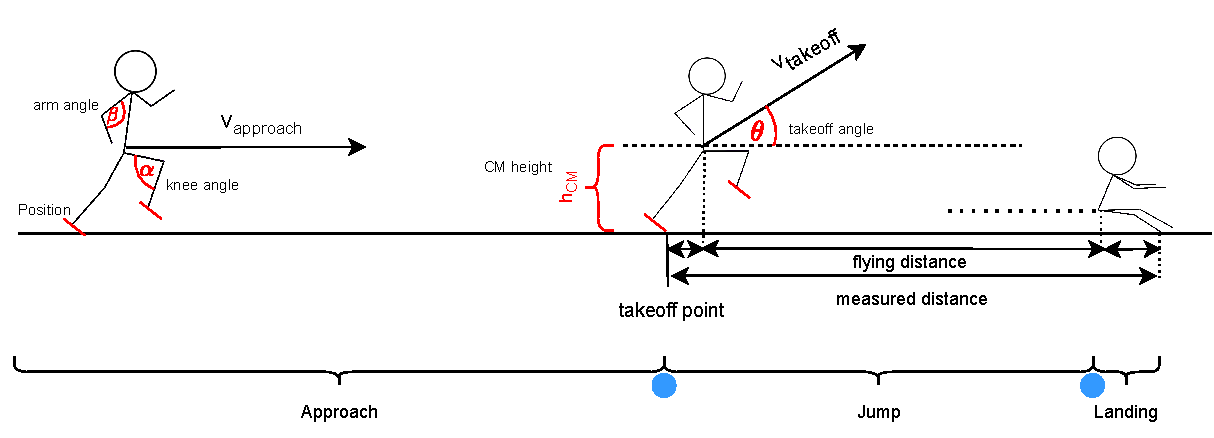
\includegraphics[scale=0.6]{long_jump_sketch.pdf}
    \caption[Long jump parameter overview]{General long jump overview.\\
    Parameters that can be analyzed are marked \textcolor{red}{red}.\\
    \textcolor{cyan}{$TP_0$} and \textcolor{cyan}{$TP_1$} denote phase
    transition points.}
    \label{fig:4_long_jump_sketch}
\end{figure}
\FloatBarrier

\subsection{Video processing}\label{subsec:4_body_keypoint_detection}
After a video has been recorded, several processing steps need to be performed
to calculate the parameters shown in \autoref{fig:4_long_jump_sketch}.
All calculations are performed for each input video frame respectively.
In the first processing stage, multiple filters can be applied to each frame.
The body key point detection is then performed on the filtered output. 
Based on these key points, the jumping parameters can be calculated which are
then in a last stage saved to a hdf5 file as well as used for the automatic
takeoff frame detection.\\
The whole process is visualized below in \autoref{fig:4_video_pipeline}.
\begin{figure}[!h]
    \centering
    \includegraphics[scale=0.54]{video_pipeline.pdf}
    \caption[Video processing pipeline]{Video processing pipeline.\\
    Stages, that each video frame passes through.}
    \label{fig:4_video_pipeline}
\end{figure}
\FloatBarrier
\noindent In the following subsections each of the shown processing stages
will be explained in detail.

\subsubsection*{Pre-processing via filter application}\label{subsubsec:4_filter_processing}
The first stage is meant to prepare the incoming video frames to get the best
possible result from the following pose detection stage.
Thus, this stage will in the following be referred to as \textit{pre
processing stage}.\\
To get an accurate pose detection result it is important to have sharp edges
around the athletes' body and an overall low noise level.
This can be achieved by applying different filters to each frame.\\
Three of the most commonly used filters are high-pass (sharpening), low-pass
(blurring) and edge preserving low-pass filters, also known as bilateral
filters.
As the best choice depends on the video input and recording conditions,
all of them are implemented and can be mixed with each other.\\
The low- and high pass filter operations can be expressed as 2D spatial
convolutions of an input image \textbf{I} of size $(x_i,y_i)$ and a (quadratic)
filter kernel \textbf{K} of size $(x_k, y_k)$.
\begin{equation}
    C(i, j) = \sum_{m=-a}^{a} \sum_{n=-b}^{b} K(m, n) \cdot I(i - m, j - n)
\end{equation}   
where C is the filtered output frame, $a = \lfloor \frac{x_k}{2} \rfloor$ and
$b = \lfloor \frac{x_i}{2} \rfloor$.
This method is also known as moving window filtering and is supported by
opencv using the \texttt{filter2D()} method.\\
The low pass filter especially helps to reduce noise in an input video frame.
Because of its' blurring character, the edges around the athletes' body lose
their details as well.
However, especially in low light conditions, this can be a good first approach
to get better results from the key point detector stage.
The high pass filter on the other hand is not suitable for videos that contain
noisy frames.
The the noise would be amplified as well as the edges which leads to
a worse body key point detection performance.
However, in high quality video recordings, the high pass filter helps to
enhance the overall sharpness and therefore especially the edges around the
athletes' body.\\

\noindent To reduce the overall noise level in a video frame while preserving
edges, a third filter, namely the \textit{bilateral filter}, is implemented.
It is defined by the following equation:
\begin{equation}
    C(I)_p = \frac{1}{W_p}\sum_{q \in S}^{} {G_\sigma}_s(\lVert p - q \rVert) {G_\sigma}_r(I_p - I_q)I_q
\end{equation}
where $C(I)_p$ is the output intensity of the filtered pixel p. ${G_\sigma}_s$
is a spatial gauss filter which decreases the influence of pixel q with
increasing distance between p and q.
${G_\sigma}_r$ is a range gauss filter, meaning it decreases the influence of
pixel q with increasing intensity difference between p and q.
Their intensities are denoted as $I_q$ and $I_p$ respectively.
S represents the set of pixels close to p and is determined by a diameter d
around each pixel.
The normalization factor $W_p$ is given by:
\begin{equation}
    W_p = \sum_{q \in S}^{} {G_\sigma}_s(\lVert p - q \rVert) {G_\sigma}_r(I_p - I_q)
\end{equation}
Compared to a simple low pass filter, which is as well implemented as gaussian
filter, the bilateral filter takes advantage of not only considering the
spatial relation between a pixel and its neighbors but also the relation
between their intensity values.
This allows a bilateral filter not only to smoothen high frequencies, but to
preserve sharp edges at the same time.
Opencv offers the built-in method \texttt{bilateralFilter()} to apply a
bilateral filter to an input video frame.
Besides the frame that should be filtered, it also takes $\sigma_s$ and
$\sigma_r$ as parameters, which define the algorithms' sensitivity to
spatial- and intensity changes as well as the diameter d in pixels.\\
As the filters time complexity depends on the region around each pixel that
is taken into account in the gaussian weighting process, it is implemented as
first approach to smoothen an input video frame without losing important
details in the regions relevant for the body key point detection.

\subsubsection*{Detecting body key points}\label{subsubsec:4_detecting_body_keypoints}
Each pre processed video frame is passed to the key point detector stage.
This stage is based on the mediapipe pose detection framework (see
\autoref{subsec:2_mediapipe_framework} and \autoref{subsec:2_why_mediapipe}).
The models used in this work are the BlazePose models.
BlazePose is a convolutional neural network with an architecture similar to
MobileNetV2.\\
It is capable of detecting a total of 33 body key points (shown in
\autoref{fig:2_body_keypoints}).
All of them are tried to be detected in each frame, while only few of them are
used in the following parameter calculation process.\\
The BlazePose network is able to work directly with RGB images as.
Thus, the filtered results form the pre-processing stage are as well in the
RGB color space.
The output generally is a 5-tuple for each detected key point.
Besides \texttt{x and y} coordinates, BlazePose also offers a
\texttt{depth estimation} and values describing the probability of a key point
being \texttt{present} and \texttt{visible} in the current frame.
The x and y values are normalized according to the image width and height.
Furthermore, BlazePose offers three different models\footnote{light, full and
heavy} which differ in the amount of parameters, thus in the networks'
complexity and the resulting detection accuracy.
Their inference times range from 0.02s to 0.25s per input video frame
respectively.
Hence, the least complex model can also be used for real time pose detection.\\
This project supports all three models, as a quick and less accurate analysis
can be sufficient (especially in good lighting and recording conditions),
whereas the best detection results, especially in poor quality videos are
achieved by using the heavy model.\\
The detected poses can be visualized as can be seen in following
\autoref{fig:4_pose_detection_in_out}: 
\begin{figure}[h!]
    \begin{subfigure}[b]{0.47\textwidth}
        \includegraphics*[scale=0.1]{takeoff_good.png}
        \caption{Sample input frame}
        \label{subfig:input_frame}
    \end{subfigure}
    \hfill
    \begin{subfigure}[b]{0.5\textwidth}
        \includegraphics*[scale=0.185]{takeoff_keypoints.png}
        \caption{Pose detection output}
        \label{subfig:output_pose_detection_result}
    \end{subfigure}
    \caption[Pose detection example]{Sample pose detection output.\\
    (a) is the input video frame and (b) is the pose detector output.
    The input frame was pre processed using a high pass filter.}
    \label{fig:4_pose_detection_in_out}
\end{figure}

\subsubsection*{Arm- and knee angle calculation}
Based on the previously detected body key points, the parameters shown in
\autoref{fig:4_long_jump_sketch} can be calculated.
Especially knee angles during the run up- and takeoff phase can give important
insights into an athletes' overall jumping dynamics.
In this context, lower knee angles during the run up (at the toe-off point) as
well as during the takeoff (swing leg) were found to lead to better jumping
results\cite{mattes_kinematic_2021}.
Thus, these parameters are calculated by the software and can be saved and
visualized afterwards.\\
In the following, the angle calculation is explained based on the knee angle
calculation.
Taking the relevant detected key points into consideration, following
situation is given:
\begin{figure}[!h]
    \centering
    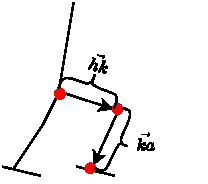
\includegraphics[scale=0.9]{knee_angles_calc.pdf}
    \caption[Knee angle calculation]{Knee angle calculation and related body
    key points.\\
    \textcolor{red}{Red dots} represent the body key points needed to calculate
    the knee angle. $\vec{hk}$ and $\vec{ka}$ denote the hip-knee vector and
    the knee-ankle vector respectively.}
    \label{fig:4_knee_angle_calculation}
\end{figure}
\FloatBarrier
\noindent The vectors $\vec{hk}$ and $\vec{ka}$ can be calculated using the
detected key points' coordinates:
\begin{equation}\label{eq:knee_angle_vectors}
    \vec{hk} = \begin{bmatrix}
        knee.x - hip.x \\
        knee.y - hip.y
    \end{bmatrix} \\
    \text{\ and \ }
    \hfill
    \vec{ka} = \begin{bmatrix}
        ankle.x - knee.x \\
        ankle.y - knee.y
    \end{bmatrix}
\end{equation}
\noindent Where .x and .y denote the key points' respective x and y coordinates.\\
The knee angle $\theta_{knee}$ is then represented by the angle
between $\vec{hk}$ and $\vec{ka}$ and can be calculated by using the scalar
product of $\vec{hk}$ and $\vec{ka}$ and their norms (lengths):
\begin{equation}\label{eq:knee_angle}
    \theta_{knee} = \arccos\left(\frac{\vec{hk} \cdot \vec{ka}}{\lvert \vec{hk} \rvert \cdot \lvert \vec{ka} \rvert}\right)
\end{equation}
where $\cdot$ defines the scalar product in this case.
The scalar product and the norm are calculated using numpys'
\texttt{dot()} and \texttt{norm()} methods.\\
The arm angle calculation is performed analogously and is therefore not shown
in detail.\\
As the knee- and arm angle calculations have to be done for each video frame,
they have to be implemented efficiently not to negatively influence the
overall analysis time.
Thus, numpy is used to perform the calculations.
\begin{pythoncode}[caption=Angle calculation,label=alg:angle_calc_algo]
    def calc_angle(first_vec, second_vec):
        first_vec_norm = np.linalg.norm(first_vec)
        second_vec_norm = np.linalg.norm(second_vec)
        if first_vec_norm == 0 or second_vec_norm == 0:
            return np.nan
        return 180 - np.rad2deg(
            np.arccos(
                (np.dot(first_vec, second_vec))
                / (first_vec_norm * second_vec_norm)
            )
        )
\end{pythoncode}
The above shown \texttt{calc\_angle()} function takes the two vectors as
arguments between which the angle should be calculated.
These vectors are, in case of the arm- and knee angles, directly given by the
detected body key point positions (see
\autoref{subsubsec:4_detecting_body_keypoints} and
\autoref{eq:knee_angle_vectors}).\\
%TODO%
By using this implementation, the overall angle calculation is sufficient fast
(performance analysis are shown in \autoref{subsec:4_runtime_performance})
in comparison to the keypoint detection process in order to allow for a quick
on-field analysis.

\subsubsection*{Takeoff angle calculation}
As can be seen in \autoref{fig:4_long_jump_sketch}, in the moment of the
takeoff, the \ac{CM}'s vertical velocity changes its direction rapidly.
This change can be quantised by the angle around which the overall
velocity vector rotates.
The calculated angle is in the following referred to as \textit{takeoff angle}
which is one of the most important pre-jump parameters.
As shown in~\cite{seyfarth_optimum_2000}, even small deviations of around
1\textdegree\ of the optimal takeoff angle can lead to shorter measured
distances (see \autoref{fig:4_long_jump_sketch}) of up to 5~cm.
The optimum takeoff angle differs between athletes and is especially
correlated to the takeoff speed~\cite{tsuboi_mathematical_2010-1}.\\
To calculate the takeoff angle, two vectors are needed.
The first vector is a horizontal vector origin in the athletes \ac{CM}.
The second vector represents the athletes'velocity, which, in this case, 
is considered equal to their \ac{CM}'s velocity.
This vector is calculated based on the takeoff frame, which needs to be
determined first (see \autoref{subsec:4_takeoff_detection}).
The second frame which is used to calculate the velocity vector is chosen
according to an offset f based on the videos' frame
rate\footnote{Chosen as $\frac{1}{10}$th of the frame rate}.
The \ac{CM}'s velocity vector is therefore given by:
\begin{equation}
    \vec{{}v}_t = \frac{1}{f} * (\vec{{}x}_{t+f} - \vec{{}x}_t)
\end{equation}
where f is the frame offset and $\vec{{}x}_i$ are the position vectors.
Here, $\vec{{}x}_t$ represents the \ac{CM} position at the moment of the takeoff
whereas $\vec{{}x}_{t+f}$ denotes the \ac{CM} position f frames later.\\
\autoref{eq:knee_angle} can then be applied again yielding following equation
for the takeoff angle:
\begin{equation}\label{eq:takeoff_angle}
    \theta_{\text{takeoff}} = \arccos\left(\frac{\vec{v_t} \cdot \vec{h_t}}{\lvert\vec{v_t}\rvert \cdot \lvert\vec{h_t}\rvert}\right)
\end{equation}
where $\vec{h_t}$ denotes any horizontal vector, e.g. $\vec{h_t} = [1, 0]$.\\
\autoref{eq:takeoff_angle} is calculated by using the function shown in
\autoref{alg:angle_calc_algo} by passing the two vectors shown in following
\autoref{fig:4_takeoff_angle_calculation}:
\begin{figure}[!h]
    \centering
    \begin{subfigure}{0.45\textwidth}
        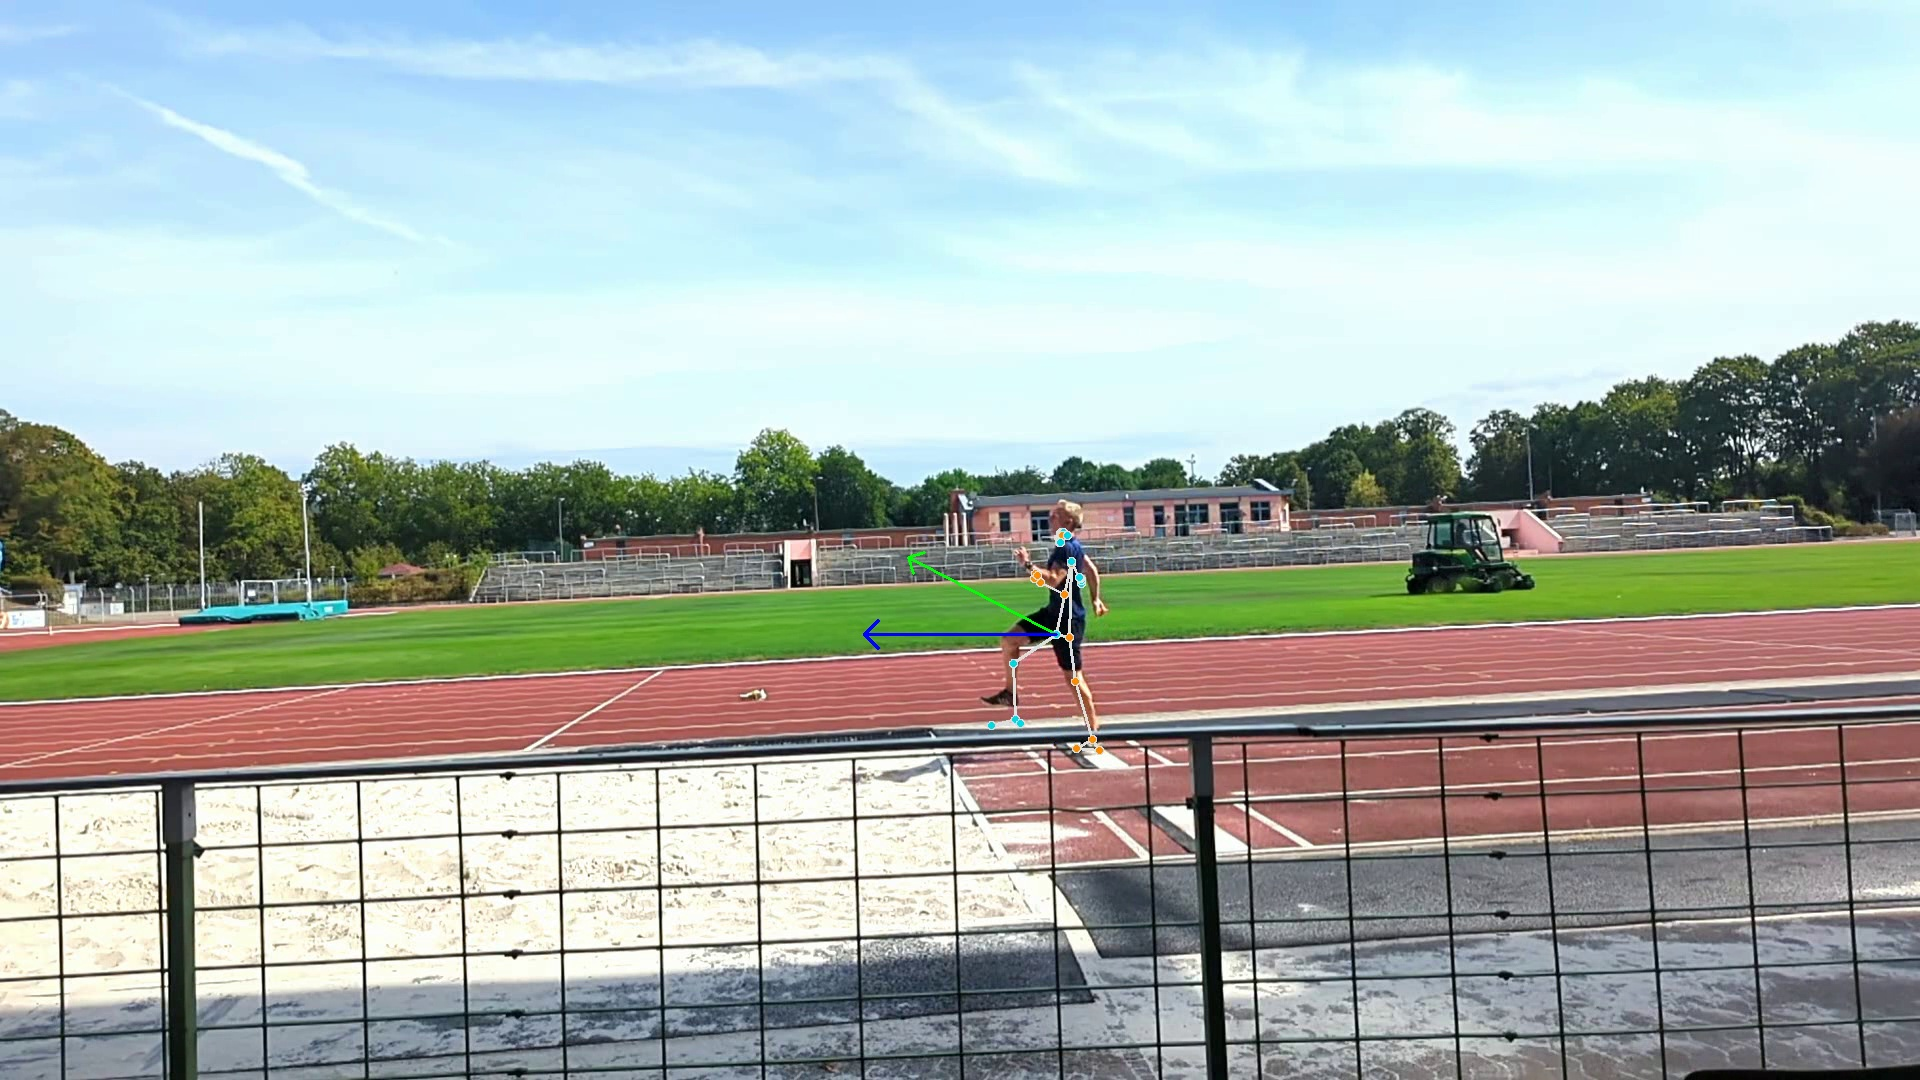
\includegraphics[scale=0.1]{takeoff_angle_overlay.jpg}
        \caption{Poses shown as overlay}
    \end{subfigure}
    \begin{subfigure}{0.45\textwidth}
        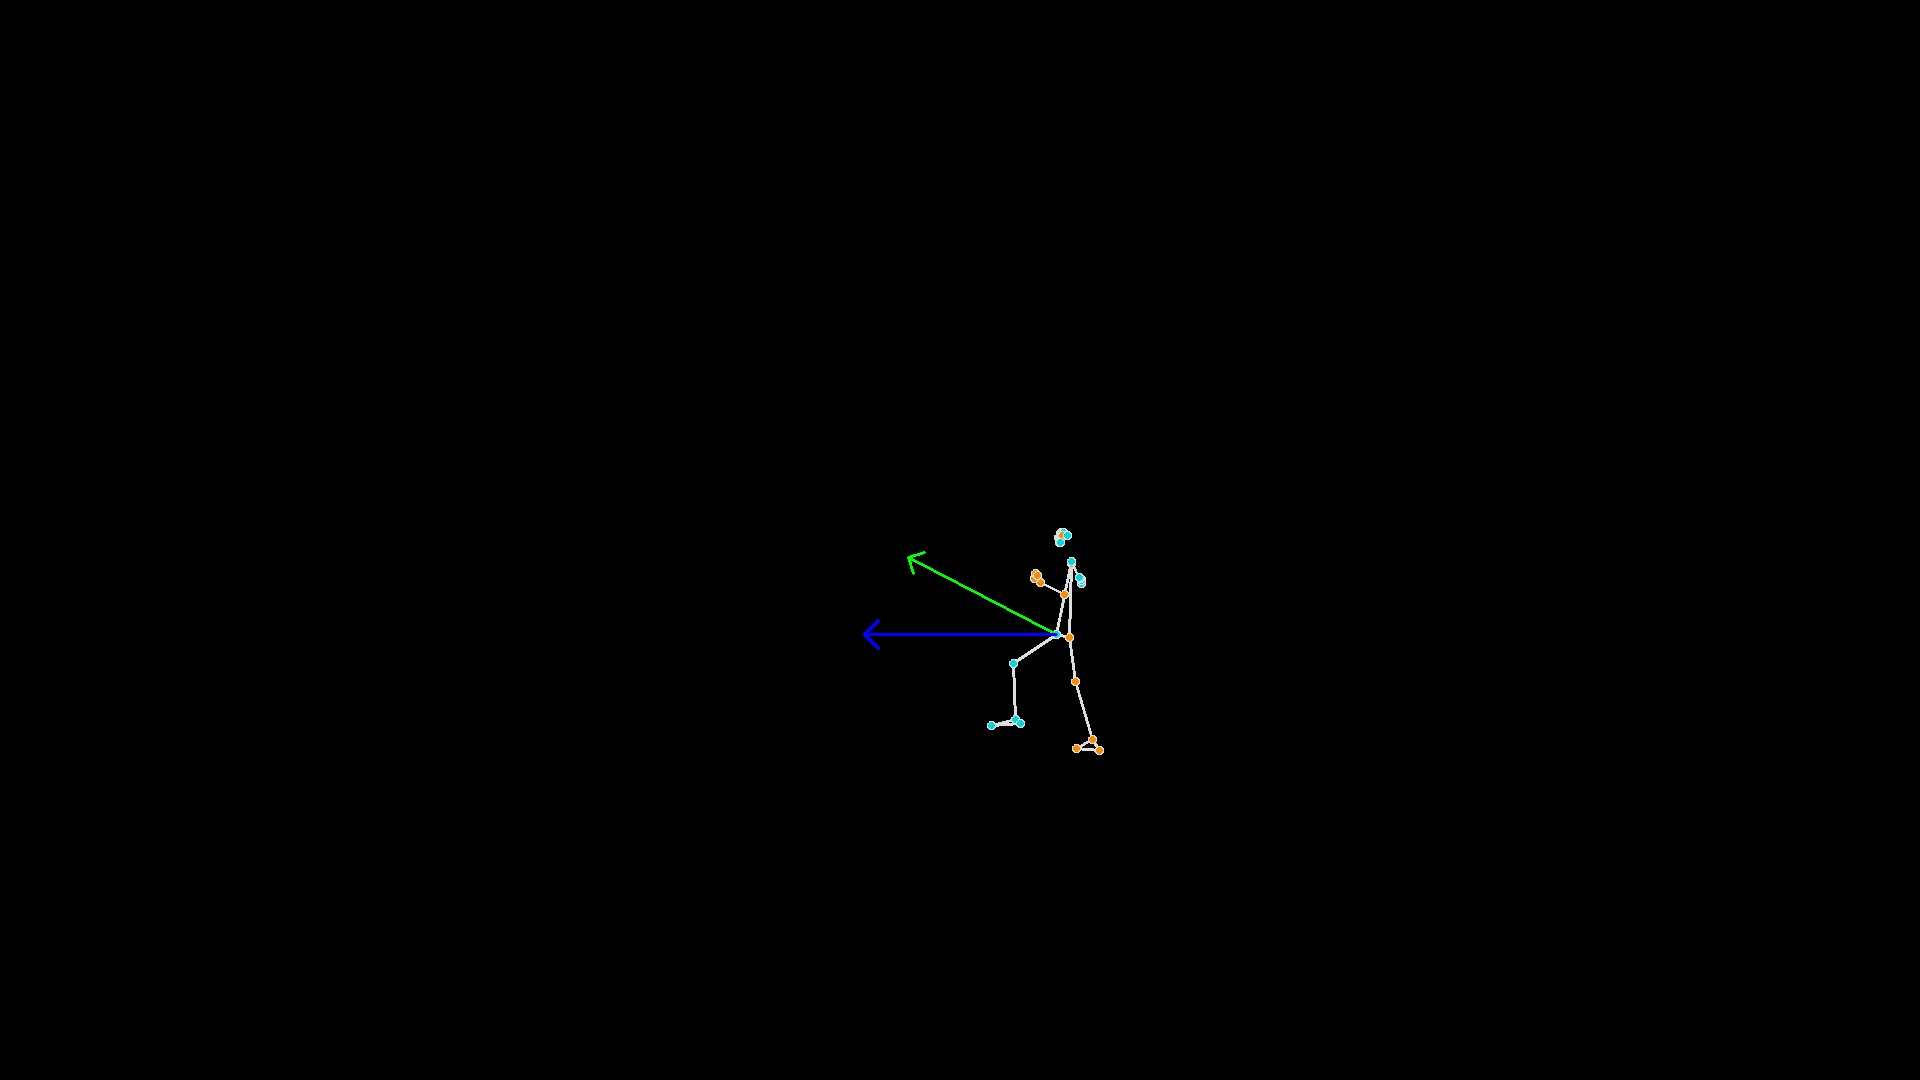
\includegraphics[scale=0.1]{takeoff_angle_no_overlay.jpg}
        \caption{Extracted vectors and positions}
    \end{subfigure}
    \caption[Takeoff angle]{Takeoff frame annotated with the
    \textcolor{green}{two vectors} that define the takeoff angle marked
    green.\\}
    \label{fig:4_takeoff_angle_calculation}
\end{figure}
\FloatBarrier
\noindent The horizontal vector in above \autoref{fig:4_takeoff_angle_calculation}
represents $\vec{h_t}$ in \autoref{eq:takeoff_angle} and the other vector
visualizes $\vec{v_t}$ respectively.
Moreover, the velocity vector is scaled by a factor of 20 due to visualization
reasons.\\

\subsection{Automatic takeoff frame detection}\label{subsec:4_takeoff_detection}
Generally, a long jump can be divided into three different phases, namely
approach, jump and landing.
In \autoref{fig:4_long_jump_sketch}, an overview of the phases is presented,
with the takeoff phase denoted by the first phase transition point ($PT_0$).\\
Of all phases, understanding the dynamics of the takeoff phase is especially
important, as it represents the last opportunity for an athlete to actively
influence critical jumping conditions (e.g.\ takeoff speed, takeoff angle,
\dots).
Within this short\footnote{0.1s - 0.2s\cite{mechanical_power_long_jump}} time
period the initial kinetic run-up energy is mostly transformed into elastic
energy\cite{wittersModelElasticTake1992}.\\
Moreover, the velocity vector of an athletes' \ac{CM} changes its direction
in the moment of the takeoff\cite{murakiJointTorquePower2008}, as illustrated in
\autoref{fig:4_long_jump_sketch}.
The forces produced during the takeoff strongly influence the resulting
jumping distance\cite{hayCitiusAltiusLongius1993}.\\
Due to the short time period a takeoff takes, it can be difficult to detect
the takeoff frame in a long jump video in order to be able to analyze the
exact pre-jump conditions.\\\\
However, especially to allow for an on-field jumping analysis, a quick takeoff
frame detection is crucial.
Thus, an algorithm that can automatically detect the takeoff frame in a long
jump video is implemented in the following.\\\\
The identification of the takeoff frame relies solely on the video input.
This means, the takeoff point has to be derived by analyzing (a combination
of) the parameters listed in \autoref{sec:4_analysis_software}.
Additionally, arm angles (and position) are not considered to be of great
interest to detect the takeoff in the following.
Therefore, the left- and right foot positions, both knee angles and the
position of the \ac{CM} are analyzed in pre-recorded long jump videos of male
long jumpers at different professional levels reaching from hobby- to Olympian
athlete.
The analyzed videos differ in their length and quality as well as in the
jumping part they show (e.g.\ some videos do not show the full run-up).
The results of three exemplary analysis are presented in
\autoref{fig:4_angles_height_plot}.
The best suitable parameter for the takeoff frame detection is selected based
on these analysis results.
To compare\footnote{Regarding their suitability as takeoff frame indicators}
the various analyzed parameters, the takeoff frame was initially manually
selected (highlighted as a \textcolor{blue}{blue vertical line} in each
analysis within \autoref{fig:4_angles_height_plot}).\\
The presented data has not been cleaned up in any way.
This can especially be seen in the first and last analysis, in which the
position and angle data is not accurate due to body key point detection
inaccuracies.
These inaccuracies however are not of great interest at this point as the key
points are detected correctly during the approach after a few frames.\\\\
In each analysis the left and right foot positions as well as the
according knee angles interchange from step to step.
The relative \ac{CM} height remains on the same level during the approach.\\
Behind the takeoff point, the relative hip- and foot heights increase quickly
until the maximal height is reached and the landing phase starts.
Moreover, the swing legs' foot height increases faster in comparison to the
jumping legs' foot height as the latter one stays on the ground longer to
introduce the jump.\\
In the moment of the takeoff, the knee angle of the jumping leg is above 170
degree, meaning the jumping leg is fully extended.
The swing legs' knee angle varies in the shown examples around 100 degree.\\\\
In order to reliably detect takeoff frames, an indicator is needed that is
suitable for different video inputs and therefore especially insensitive to
different run-up and jumping techniques.  
Taking the results in \autoref{fig:4_angles_height_plot} into consideration,
it can be noted that all analyzed positions (left-/ right foot and \ac{CM})
rapidly change their height after the takeoff.
However, as the \ac{CM}'s position is more stable in all shown analysis, it is
chosen over the foot positions as first takeoff indicator.
The second indicator is based on the jumping legs' full extension during the
takeoff.
Thus, it is chosen as a combination of both knee angles.\\\\
The following takeoff frame detection is therefore based on both selected
indicators (\ac{CM} height and knee angles).
The primary indicator is chosen as the \ac{CM} height, while the knee angles
are chosen as secondary indicator.\\
To detect the takeoff based on the primary indicator, a mathematical
description of the \ac{CM} trajectory is modelled using multiple regressions
which allows for analytically determining the takeoff point.
The secondary indicator is then used to verify the found takeoff frame.
In particular, a the takeoff frame is only considered to be correctly
identified if the corresponding (jumping leg's) knee angle is above
$170^{\circ}$.\\
The process is explained in detail in the following.

\begin{figure}[h!]
    \begin{subfigure}[b]{0.5\textwidth}
        \includegraphics*[scale=0.45]{jump_runup_poor_start.png}
        \captionsetup{justification=centering, singlelinecheck=false, labelfont=bf}
        \label{subfig:runup_jump_landing_height}
    \end{subfigure}
    \begin{subfigure}[b]{0.5\textwidth}
        \includegraphics*[scale=0.45]{jump_runup_poor_start_angles.png}
        \label{subfig:runup_jump_landing_angles}
    \end{subfigure}
    \begin{subfigure}[b]{0.5\textwidth}
        \includegraphics*[scale=0.45]{jump_no_runup.png}
        \label{subfig:no_runup_height}
    \end{subfigure}
    \hfill
    \begin{subfigure}[b]{0.5\textwidth}
        \includegraphics*[scale=0.45]{jump_no_runup_angles.png}
        \label{subfig:no_runup_angles}
    \end{subfigure}
    \begin{subfigure}[b]{0.5\textwidth}
        \includegraphics*[scale=0.45]{jump_runup_poor.png}
        \label{subfig:runup_jump_height}
    \end{subfigure}
    \begin{subfigure}[b]{0.5\textwidth}
        \includegraphics*[scale=0.45]{jump_runup_poor_angles.png}
        \label{subfig:runup_jump_angles}
    \end{subfigure}
    \caption[Analyzed jumping parameters over time]{Analyzed and calculated
    jumping parameters over time.\\
    \textbf{Left column}: Analyzed left / right foot height and hip height.\\
    \textbf{Right column}: Calculated knee angles over time.\\
    The \textcolor{blue}{vertical lines} represent the visually selected
    takeoff point.\\
    \textbf{First row}: full run-up, full jump.\ \textbf{Second Row}: short 
    run-up, full jump.
    \textbf{Third row}: full run-up, full jump, poor video quality}
    \label{fig:4_angles_height_plot}
\end{figure}
\FloatBarrier

\subsubsection{Regression}
As the takeoff point detection is based on linear and quadratic regression,
both are briefly introduced in the following.
Regression generally describes the approximation of a polynomial function to
fit a given dataset.
The dataset that is tried to be approximated in this case is the height of the
\ac{CM}.
The dataset can be expressed as (T, H), where H holds the heights of the
\ac{CM} and T holds the related time points.
As the input is a video, T represents a simple vector holding the
video's frame numbers.
For the following steps it is helpful to express T and H as column vectors:
\begin{equation}
    \vec{t} = \begin{bmatrix}
        1\\
        2\\
        \vdots\\
        n
    \end{bmatrix}
        \quad\text{and}\quad
    \vec{h} = \begin{bmatrix}
        h_1\\
        h_2\\
        \vdots\\
        h_n
    \end{bmatrix}
\end{equation}
where n is the total number of video frames and $h_i$ is the $i\--th$ recorded
height of the \ac{CM}.\\
Taking the \ac{CM} in \autoref{fig:4_angles_height_plot} into consideration,
a whole jump can hardly be fitted with a single polynomial function.
However, as shown in \autoref{fig:4_long_jump_sketch}, a long jump consists of
multiple phases.\\
This offers an opportunity to detect the takeoff.
As mentioned before, the takeoff frame is defined as the point where the
approach phase ends and the jumping phase starts, ($PT_0$ in
\autoref{fig:4_long_jump_sketch}).
Thus, if a mathematical expression can be found for each phase respectively,
the takeoff frame is found implicitly.
The algorithm used for this task is based on the algorithm for a takeoff
frame detection developed by Muniz \cite{muniz_detection_2019}.\\
Other than supposed in his work, the detection algorithm in this work is not
based on the foot positions, but on the \ac{CM} position.
There are several reasons for preferring the \ac{CM} over the foot positions.
One of the most important reasons lies in the different jumping techniques,
more specifically in the resulting differences during the jumping phase.
While the foot path during the jumping phase is rather smooth for
athletes using the \textit{hang technique}, it is very different for
athletes using the \textit{hitch-kick technique}.
Latter one is characterized by quick foot position interchanges, making it
more error-prone for inaccuracies in the corresponding body key point
detection.
Thus, approximating the jumping phase based on the foot positions is more
complex and less precise.
The \ac{CM} however follows a similar path independent from the jumping
technique, making it more suitable for the given purpose of detecting the
takeoff frame.\\\\
\noindent In the following, the algorithm is explained in detail.
All mentioned frame numbers and jumping phases refer to
\autoref{fig:4_long_jump_sketch}.\\
The runup phase includes all frames in the interval $[0, PT_0[$, the jumping
phase is covered by the frames in range $[PT_0, PT_1[$ and the landing phase
is shown by the frames in the interval $[PT_1, n[$, where $PT_0$ defines the
first Phase Transition point (the takeoff) and $PT_1$ the point at which the
landing phase starts.
Each phase by itself can be approximated by a polynomial function.
The approach and the landing can be fitted using a linear expression.\\
Thus, two linear regressions are performed separately to find two expressions
of the form
\begin{equation}\label{eq:linear_function}
    \\y = \beta_0 + \beta_1t
\end{equation}
which directly yields following linear regression function:
\begin{equation}\label{eq:linear_reg_function}
    \\y_i = \beta_0 + \beta_1t_i + \epsilon_i
    \quad\quad
    i = \text{start},\ \dots\ ,\text{end}
\end{equation}
where $\beta_0$ and $\beta_1$ are the coefficients that need to be found.
start and end represent the first and last frame index that should be
considered in the linear regression.
For the approach phase this leads to $start = 0$ and $end = TP_0 - 1$, the
landing phase is accordingly represented by $start = TP_1$ and $end = n - 1$.\\
\autoref{eq:linear_reg_function} can also be expressed as matrix equation:
\begin{equation}\label{eq:linear_reg_matrix}
    \underbrace{
    \begin{bmatrix}
        y_0\\
        y_1\\
        \vdots\\
        y_r\\
    \end{bmatrix}}_{\substack{\vec{y}}}
    =
    \underbrace{
    \begin{bmatrix}
        1 & t_{\text{start}}\\
        1 & t_{\text{start} + 1}\\
        \vdots & \vdots\\
        1 & t_{\text{end}}
    \end{bmatrix}}_{\substack{\text{Design matrix} \\ T}}
    \underbrace{
    \begin{bmatrix}
        \beta_0\\
        \beta_1
    \end{bmatrix}}_{\substack{\text{Coefficients} \\ \text{vector} \\
    \vec{\beta}}}
    +
    \underbrace{
    \begin{bmatrix}
        \epsilon_0\\
        \epsilon_1
    \end{bmatrix}}_{\substack{\text{Error} \\ \text{vector} \\
    \vec{\epsilon}}}
\end{equation}
where $r = end - start$.
This can be written in short form as:
\[
    \vec{y} = T\vec{\beta} + \vec{\epsilon}    
\]
Now, the vector $\vec{\beta}$ needs to be found that minimizes the sum of
errors $E_{SSE}$ between the measured \ac{CM} heights $h_i \in \vec{h}$ and
the fitted polynomial $y_i$ at time step i.
To measure the error, the \ac{SSE} is used:
\begin{equation}
    E_{SSE} = \sum_{i=start}^{end} \epsilon_i^2 = \sum_{i=start}^{end} (h_i - y_i)^2
\end{equation}
Using the simple linear expression from \autoref{eq:linear_reg_function},
following error function is found:
\begin{equation}
    E_{SSE} = \sum_{i=start}^{end} (h_i - \beta_0 - \beta_1i)^2
\end{equation}
By using the matrix notation introduced in \autoref{eq:linear_reg_matrix},
the equation above can be written in matrix notation as well:
\begin{equation}\label{eq:sse_matrix}
    E_{SSE} = (T\vec{\beta} - \vec{h})^T(T\vec{\beta} - \vec{h})
\end{equation}
As $\vec{\beta}$ should minimize $E_{SSE}$, the minimum of $E_{SSE}$ is
needed, which can be found by solving following equation:
\begin{equation}\label{eq:gradient_linear_case}
    \nabla_{\vec{\beta}}E_{SSE} = \nabla_{\vec{\beta}}(T\vec{\beta} - \vec{h})^T(T\vec{\beta} - \vec{h}) = 0
\end{equation}
where $\nabla_{\vec{\beta}}$ denotes the gradient with respect to $\vec{\beta}$.\\
The coefficients can then be found by solving
\autoref{eq:gradient_linear_case} for $\vec{\beta}$, which yields the 
following normal equation:
\begin{equation}\label{eq:normal_equation}
    \vec{\beta} = (T^T T)^{-1}(T^T\vec{h})
\end{equation}
that especially requires $(T^{T} T)$ to be invertible.
A proof of \autoref{eq:normal_equation} can be found in
\cite{proof_linear_regression_mat}.\\
As mentioned, this process is performed twice to find a linear approximation
for the approach and the landing phase of an athletes' \ac{CM} respectively.\\\\
The jumping phase cannot be approximated with a linear polynomial.
However, as can be seen in \autoref{fig:4_angles_height_plot} after the marked
takeoff point, the curve of the \ac{CM} height can be approximated using a
parabola.
Thus, a quadratic regression is used to find a curve that describes the height
of the \ac{CM} during the jumping phase.
The second order polynomial that needs to be found is of the form:
\begin{equation}\label{eq:quadratic_function}
    \\y = \beta_0 + \beta_1t + \beta_2t^2
\end{equation}
yielding the quadratic regression function:
\begin{equation}\label{eq:quadratic_reg_function}
    \\y_i = \beta_0 + \beta_1t_i + \beta_2t_i^2 + \epsilon_i
    \quad\quad
    i = PT_0,\ \dots\ ,PT_1 - 1
\end{equation}
$PT_0\ \text{and}\ PT_1$ are the phase transition points shown in
\autoref{fig:4_long_jump_sketch}.
The following steps are equal to the linear regression shown above.
Thus, only the differences are shown in detail.\\
The T matrix in \autoref{eq:linear_reg_matrix} contains all frame
numbers as column vector.
Because a linear relation was tried to be found to approximate the approach
and  landing phase before, the T matrix as well only contained linear values.
Now however, a quadratic relation needs to be found.
Thus, the T matrix needs to be extended by one more column holding the
quadratic frame numbers yielding following matrix equation:
\begin{equation}\label{eq:quadratic_reg_matrix}
    \underbrace{
    \begin{bmatrix}
        y_0\\
        y_1\\
        \vdots\\
        y_r\\
    \end{bmatrix}}_{\vec{y}}
    =
    \underbrace{
    \begin{bmatrix}
        1 & t_{PT_0} & t_{PT_0}^2\\
        1 & t_{PT_0 + 1} & t_{PT_0 + 1}^2\\
        \vdots & \vdots & \vdots\\
        1 & t_{PT_1 - 1} & t_{PT_1 - 1}^2
    \end{bmatrix}}_{T}
    \underbrace{
    \begin{bmatrix}
        \beta_0\\
        \beta_1\\
        \beta_2
    \end{bmatrix}}_{\vec{\beta}}
    +
    \underbrace{
    \begin{bmatrix}
        \epsilon_0\\
        \epsilon_1\\
        \epsilon_2
    \end{bmatrix}}_{\vec{\epsilon}}
\end{equation}
where $r = PT_1 - 1 - PT_0$.
The error function which needs to be minimized can be set equivalent to the
linear case (\autoref{eq:sse_matrix}).
Comparing \autoref{eq:linear_reg_matrix} and \autoref{eq:quadratic_reg_matrix}
the only things that change are the number of coefficients (and thus the
number of error terms) as well as the design matrix T, which holds one more
column.
The steps to determine the coefficients $\vec{\beta}$ are equal to the linear
case in equations~\ref{eq:sse_matrix} to~\ref{eq:normal_equation}.
$\vec{\beta}$ is then given by the same normal equation~
\ref{eq:normal_equation} as in the linear case:
\[
    \vec{\beta} = (T^T T)^{-1}(T^T\vec{h}) 
\] 
where $\vec{\beta}$ contains three coefficients $\beta_0$, $\beta_1$ and
$\beta_2$ to approximate the jumping phase.\\\\

\noindent By using this linear- and quadratic regression approach, the whole
jump can be modelled mathematically.
However, in order to find the best fitting model, the phase changing points
($PT_0$ and $PT_1$ in \autoref{fig:4_long_jump_sketch}) need to be determined.
This can be done by minimizing the overall error $E_{total}$, which is defined
as the sum of regression errors resulting from the three independent
regressions performed (one per jumping phase):

\begin{equation}\label{eq:total_error}
    E_{total} = E_{approach} + E_{jump} + E_{landing}
\end{equation}

\noindent $E_{total}$ can be minimized by using a brute-force approach.
For each possible combination of phase transition points, two linear
regressions (representing approach and landing) and one quadratic regression
(representing the jumping phase) are performed and their individual errors
given by \autoref{eq:sse_matrix} are summed up.
The combination of phase transition points that leads to the minimal
$E_{total}$ is then considered as the optimal model to fit the overall jump.
As the found phase transition points directly represent their corresponding
frame numbers, the takeoff frame is directly given by the first phase
transition point.\\
The described process is outlined in following
Algorithm~\ref{alg:takeoff_frame}.
\begin{algorithm}[h!]
    \caption{takeoff\_frame(cm\_height: array, knee\_angles: array)}
    \begin{algorithmic}[1]
        \State $n \gets \text{length of } cm\_height$
        \State $total\_error \gets \text{initial error}$
        \State $transition\_points \gets (0,0)$
        \For{$i \gets 0$ \textbf{to} $n - 1$}
            \For{$j \gets i + 1$ \textbf{to} $n$}
            \State $\vec{\beta_{approach}}, error\_approach \gets \text{lin\_reg}(hip\_height[:i])$
            \State $\vec{\beta_{jump}}, error\_jump \gets \text{quad\_reg}(hip\_height[i:j])$
            \State $\vec{\beta_{landing}}, error\_landing \gets \text{lin\_reg}(hip\_height[j:])$
            \State $fitting\_error \gets error\_approach + error\_jump + error\_landing$
                \If{fitting\_error $<$ total\_error \textbf{and} $\vec{\beta_{jump}}[0]$ $<$ 0 \textbf{and} knee\_angles[i] > 170}
                    \State $total\_error \gets$ fitting\_error
                    \State $transition\_points \gets (i,j)$
                \EndIf
            \EndFor
        \EndFor
        \State \textbf{return} transition\_points
    \end{algorithmic}
\label{alg:takeoff_frame}
\end{algorithm}
\FloatBarrier

\noindent The expression \texttt{$\vec{\beta_{jump}}[0] < 0$} guarantees, that
the found parabola for approximating the jumping phase is opened downwards.
Moreover, \texttt{$knee\_angles[i] > 170$} makes sure, that only frames in
which the knee angle is above 170 degrees can be considered as takeoff point.\\
The shown algorithms' runtime scales according to $\mathcal{O}(n^2)$
where n is the number of video frames~\footnote{in which body key points were
found}. 
Thus, it is not suitable for long video sequences.
However, as a complete long jump takes only a few seconds, the algorithm can
be used for an on-field jump analysis.\\
Algorithm~\ref{alg:takeoff_frame} was then applied to all three datasets shown
in \autoref{fig:4_angles_height_plot}. 
The results are shown in \autoref{fig:4_automatic_takeoff_results}.\\
For better understanding, the height of the \ac{CM} was extracted from the
datasets as it is the only parameter relevant for the takeoff detection.
The data is not cleaned up in any way, thus, outliers are still
visible.
However, as can be seen, the automatically detected takeoff frames are
similar to the manually annotated frame numbers.
\begin{figure}[h!]
    \centering
    \begin{subfigure}{0.45\textwidth}
        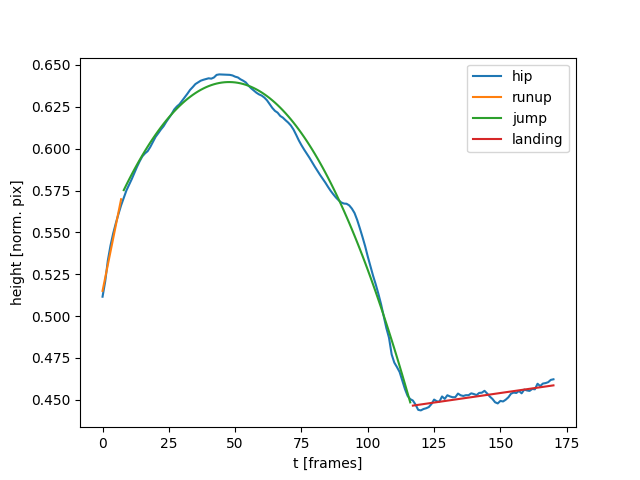
\includegraphics[width=\textwidth]{regression_jump_only.png}
        \caption{Short approach, reliable keypoint quality}
    \end{subfigure}\hfill
    \begin{subfigure}{0.45\textwidth}
        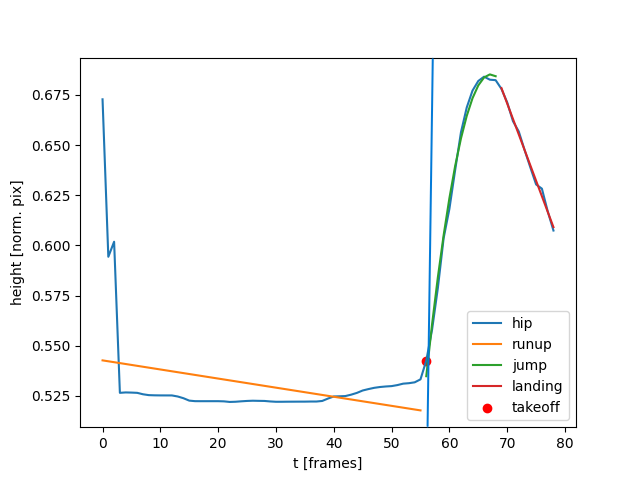
\includegraphics[width=\textwidth]{regression_poor_approach.png}
        \caption{Long approach, outliers in approach}
    \end{subfigure}
    \begin{subfigure}{0.45\textwidth}
        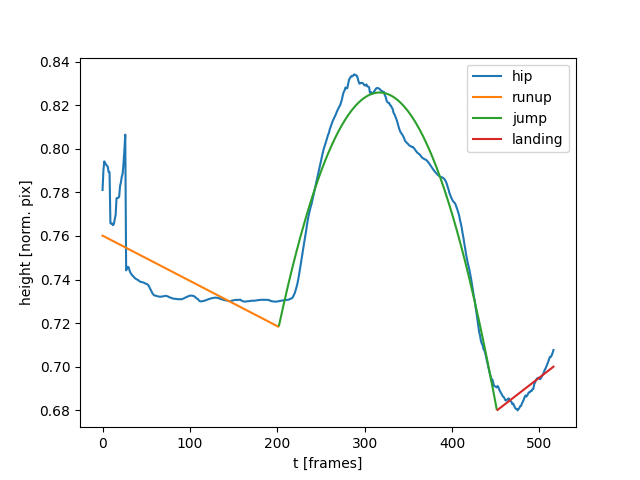
\includegraphics[width=\textwidth]{regression_poor_approach_jump.png}
        \caption{Long approach, outliers in approach and jump}
    \end{subfigure}
    \caption[Automatic takeoff frame detection results]{
        All three jumping phases approximated using linear regression
        (runup and landing) and quadratic regression (jumping phase).\\
        The automatically detected takeoff frame is marked with a
        \textcolor{red}{red dot}.\\
        The \textcolor{cyan}{vertical blue lines} represent the manually marked
        takeoff frames.}
\label{fig:4_automatic_takeoff_results}
\end{figure}
\FloatBarrier

\subsection{Saving analysis results}\label{subsec:4_param_files}
After a complete jump analysis has been performed, all data, especially
the calculated parameters such as arm- and knee angles need to be stored
permanently.
Thereby, each input video file must only be analyzed once in order to avoid
costly double analysis.
While the detected body key points are stored in form of an annotated video
file, the analysis parameters are stored alongside in a separate file which
can be re-loaded and visualized.
This file will in the following be referred to as \texttt{Parameter file}.\\
As most of the parameters are calculated frame-wise (like knee angles, foot
positions, \dots), the well-structured hdf5 file format (see
\autoref{subsec:2_hdf5}) is used for this task.
The exact file structure is shown in following 
\autoref{fig:hdf5_file_structure_param_file}:
\begin{figure}[h!]
    \centering
    \scalebox{0.8}{ % Adjust the scaling factor as needed
        \begin{minipage}{0.5\textwidth}
            \dirtree{%
            .1 Root.
            .2 \textcolor{cyan}{video\_file}.
            .2 \textcolor{cyan}{transition\_points}.
            .2 \textcolor{cyan}{takeoff\_vector}.
            .2 Frame0.
            .3 right\_foot\_x.
            .3 right\_foot\_y.
            .3 left\_foot\_x.
            .3 left\_foot\_y.
            .3 left\_knee\_angle.
            .3 right\_knee\_angle.
            .3 cm\_x.
            .3 cm\_y.
            .2 Frame1.
            .3 \dots.
            .2 Frame2.
            .3 \dots.
            .2 \dots.
        }
        \end{minipage}
    }
    \caption[HDF5 Parameter file structure]{HDF5 Parameter file structure}
    \label{fig:hdf5_file_structure_param_file}
\end{figure}
\FloatBarrier
\noindent As can be seen in above \autoref{fig:hdf5_file_structure_param_file},
each hdf5 file contains three \textcolor{cyan}{metadata} parameters.
They do not belong to a certain frame and represent important analysis results
that take several frames into consideration.
Furthermore, these parameters can be accessed efficiently.
The \texttt{transition\_points} metadata contains the phase transition points
(see \autoref{fig:4_long_jump_sketch}), whereas \texttt{takeoff\_vector} is a
tuple of the form ($\theta_{\text{takeoff}}, \vec{{}v}_t$) according to
\autoref{eq:takeoff_angle}.
As one of the shown Parameter files is created per jump analysis, an annotated
video file belongs to each of those files.
Thus, a connection to the related video file is saved in the
Parameter file in form of the \texttt{video\_file} metadata.\\
Furthermore, there is a group created for each analyzed video frame.
Within these groups there is one dataset created for each analysis parameter.\\

\noindent To allow simple and efficient read- and write operations, the class
\texttt{Parameterfile} is implemented, which abstracts the described parameter
file.
All HDF5 file interactions are implemented using the python
h5py package\cite*{collette_python_hdf5_2014}, which offers dedicated methods
for creating a whole HDF5 file as well as methods for creating groups,
datasets and metadata.\\
Taking into consideration that, for each input video frame, one group in the
according HDF5 file as well as one annotated video frame needs to be saved,
there are many memory accesses during the analysis process, which leads to
poor runtime behavior.
To reduce the number of memory accesses, the Parameterfile instances buffer
some HDF5 frame groups and then perform batch saving.
This effectively reduces the number of costly memory accesses, leading to
a better performance behavior.
The software uses a batch size of 128 by default.\\
Overall, the \texttt{Parameterfile} class manages all analysis file
interactions.
Possible interactions can be seen in its class diagram:
\begin{figure}[!h]
    \centering
    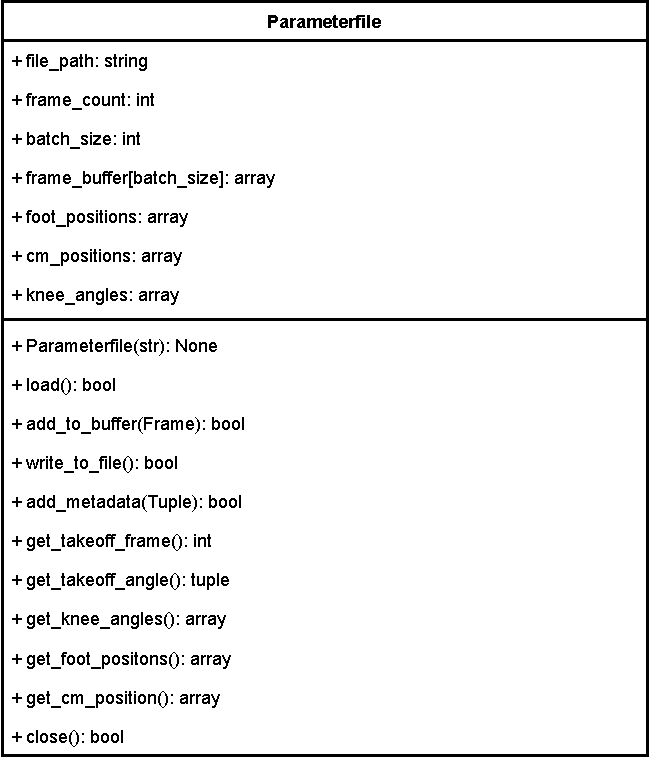
\includegraphics[scale=0.6]{Parameterfile.pdf}
    \caption[Parameterfile class diagram]{Parameterfile class diagram}
    \label{fig:4_param_file_class_diagram}
\end{figure}
\FloatBarrier
\noindent In above \autoref{fig:4_param_file_class_diagram} the
\texttt{load()} method and all \texttt{get\_x()} methods are used to retrieve
analysis parameters from saved Parameterfiles.


\subsection{Runtime considerations}\label{subsec:4_runtime_performance}
The software is mainly developed towards a high key point detection and
thus, a high parameter calculation accuracy.
However, as it is meant to be used as an on-field analysis tool, quick
analysis times are important.
Hence, in the following, some important run times are shown and discussed.\\
All following evaluations were performed on a laptop equipped with an
AMD Ryzen 5800U processor and 16GB of ram.
This setup was chosen to represent a standard setup that can be used for an
on-field analysis.\\
Generally, there are two main runtime critical parts in the jump analysis
process: first, the key point detection and second, the takeoff frame
detection.
The first one mainly depends on the users' choice of the underlying key point
detection model (evaluated later).
The latter one however performs many numerical operations.
As a result, it can potentially profit from pre-compiled implementations
using \texttt{numba} (see \autoref{subsec:3_precompile_numba}).\\
To validate this assumption some runtime comparisons based on video inputs of
10 seconds length are performed.
One is recorded at 60 \ac{FPS} and the other one at 90 \ac{FPS},
resulting in 600 and 900 frames respectively.
The results are presented in following
\autoref*{fig:takeoff_frame_detection_performance}:
\begin{figure}[!h]
    \begin{subfigure}[b]{0.48\textwidth}
        \includegraphics*[height=5cm]{absolute_runtime.png}
        \caption{Absolute runtime comparison.\\
        Error bars represent the standard deviation.}
        \label{subfig:absolute_runtime_tkf_frame}
    \end{subfigure}
    \hfill
    \begin{subfigure}[b]{0.48\textwidth}
        \includegraphics*[height=5cm]{relative_throughput.png} 
        \caption{Normalized throughput comparison.\\
        Values are directly proportional to the runtime shown in (a).}
        \label{subfig:relative_throughput_tkf_frame}
    \end{subfigure}
    \vfill
    \begin{subfigure}[b]{0.48\textwidth}
        \includegraphics*[height=5cm]{absolute_runtime_900.png}
        \caption{Absolute runtime comparison.\\}
    \end{subfigure}
    \hfill
    \begin{subfigure}[b]{0.48\textwidth}
        \includegraphics*[height=5cm]{relative_throughput_900.png} 
        \caption{Normalized throughput comparison.\\}
    \end{subfigure}
    \caption[Takeoff frame detection performance]{Runtime and throughput
    comparison between pre-compiled (\texttt{numba}) and non
    pre-compiled takeoff frame detection implementations.}
    \label{fig:takeoff_frame_detection_performance}
\end{figure}
\FloatBarrier
\noindent As can be seen, the takeoff frame detection generally scales
according to $\mathcal{O}(n^2)$, where n is the number of analyzed video
frames (explained in \autoref{subsec:4_takeoff_detection}).
Looking at a 900 frame video, this leads to $900 * 900 = 810*10^3$ loop runs.
Moreover, in each iteration, three polynomial regressions are performed which
leads to around $2.4*10^6$ regression operations.\\
Due to that many regression operations, the two evaluated implementations
differ in the way they perform the necessary regressions (see Algorithm
\ref{alg:angle_calc_algo} for details).
While the python implementation relies on \texttt{numpy}'s
polyfit\footnote{\url{https://numpy.org/doc/stable/reference/generated/numpy.polyfit.html}}
method, the pre-compiled \texttt{numba} implementation uses a custom
regression implementation which is set up according to equations
\ref{eq:linear_reg_matrix} to \ref{eq:normal_equation}.
A custom implementation is chosen, as the polyfit method offered by
\texttt{numpy} cannot be pre-compiled using \texttt{numba}.
The complete implementation is not shown, however, the main function is
presented in order to demonstrate the (simple) usage of \texttt{numba}:\\
\begin{pythoncode}[caption=Polynomial regression,label=alg:poly_fit_numba]
    import numba as nb

    @nb.jit('f4[:](f4[:], f4[:], i4)') # numba decorator
    def _fit_poly(x: np.ndarray, y: np.ndarray, deg: int):
        A = _coeff_mat(x, deg) # creates design matrix
        p = _fit_x(A, y) # solves Ax = y
        return p[::-1] # ensure p[0] to be the highest order coefficient
\end{pythoncode}
The methods \texttt{\_coeff\_mat} and \texttt{\_fit\_x} represent
\autoref{eq:linear_reg_matrix} and \autoref{eq:normal_equation} respectively.
\texttt{\_fit\_x} uses the least-squares fitting approach shown in
\autoref{eq:gradient_linear_case} to find the best fitting model.
Furthermore, the residuals (errors) which are needed (see 
\autoref{eq:total_error}) are calculated via polynomial evaluation using
Horner's method~\cite{fuentesFastEvaluationPolynomials2022}.\\
As can be seen, the only difference to a standard python function definition
is the \texttt{nb.jit() decorator} which wraps the \texttt{\_fit\_poly}
function in \texttt{numba}s' jit function to pre-compile it when the function
is first called (therefore the name \textit{Just-in-time compiler}).\\
This behavior can potentially lead to a large execution overhead before the
function can be executed for the first time.
However, numba can also pre-compile the function when the application is
launched to avoid long compiling processes during runtime.
This is achieved by passing the parameter types to numba
(\texttt{'f4[:](f4[:], f4[:], i4)'}), where f4 denotes a standard 32 bit
single precision float, i4 a standard 32 bit integer value and [:] their array
types respectively.
Moreover, the first \texttt{f4[:]} defines the functions' return type
as an array of 32 bit floats.\\
Numba needs that extra information to pre-compile the function, as the
functions' parameter types cannot be derived just by the function definition,
as python generally is a dynamically typed language.\\\\
\noindent Taking the implementations and
\autoref{fig:takeoff_frame_detection_performance} into account, the takeoff
frame detection significantly profits from the pre -compiled numba
implementation.
The absolute runtime is reduced by over 80\%, increasing the throughout by a
factor of around 5.5.
Thus, the final takeoff frame detection is implemented using \texttt{numba}s'
JIT compiler.\\\\

\noindent The other runtime crucial part is the body keypoint detection.
As aforementioned, mediapipe offers three different BlazePose keypoint
detection models differing in terms of accuracy and performance.
All three models are implemented, thus their inference times are compared.
As the final analysis will be performed on videos of size 1920 x 1080, the
performance is tested on video frames of this size.
The results are presented in following:
\begin{figure}[!h]
    \begin{subfigure}[b]{0.48\textwidth}
        \includegraphics*[height=5cm]{inference_time_models.png}
        \caption{Absolute inference time comparison.\\
        Error bars represent the standard deviation.}
        \label{subfig:absolute_inference_times}
    \end{subfigure}
    \hfill
    \begin{subfigure}[b]{0.48\textwidth}
        \includegraphics*[height=5cm]{inference_fps_models.png} 
        \caption{Theoretically achievable \acs*{FPS} comparison.\\
        Values are directly proportional to the runtime shown in (a).}
        \label{subfig:relative_inference_fps}
    \end{subfigure}
    \caption[Inference time comparison]{Inference time comparison of all three
    mediapipe pose detection models.}
    \label{fig:mp_model_inference_time_comparison}
\end{figure}
\FloatBarrier
\noindent As can be seen in above \autoref{fig:mp_model_inference_time_comparison}
the inference times significantly differ between the three BlazePose pose
detection models.
While the full, thus most complex and most accurate detection model achieves
speeds of up to around 10~\ac{FPS}, the light model can evaluate up to
40~\ac{FPS}.
This means latter one can theoretically even be used as a real time analysis
option for video recordings at 30~\ac{FPS}.
However, as this work focuses on the video analysis, the real time
capabilities are not part of this works' scope.\\
The parameter calculation (see \autoref*{sec:4_analysis_software}) is
neglected in the runtime measurements, as they are much less computational
expensive compared to the body key point detection and the takeoff frame
detection.\\
Thus, a full long jump video of 10~sec lengths (60~\ac{FPS}) can be fully
analyzed in around a minute.

\subsection{Visualization in a \acs*{GUI}}\label{subsec:4_lj_software_gui}
To present the jump analysis, a \ac{GUI} is implemented.
This \ac{GUI} is mainly developed regarding three purposes:
\begin{enumerate}
    \item Choose video files and analysis parameters.
    \item Present analysis results while the analysis is running.
    \item Present the fully analyzed video and the calculated parameters. 
\end{enumerate}
\noindent In the following, the \ac{GUI} will be shown and explained in two
steps.
At first, the first two points in above listing will be shown
and secondly, the full analysis visualization is presented.\\\\
\noindent The second point allows an athlete (or trainer) to analyze \textit{
single frame parameters} while the video is still being evaluated.
Single frame parameters are those, that do not need all frames to be evaluated
but just rely on the current frame (e.g. knee angles and arm angles).
In contrast a full analysis includes all other parameters, such as the takeoff
frame and the takeoff angle.
This allows to reduce the actual on-field analysis times, as a first overall
jumping impression can be offered immediately.\\
The \ac{GUI} that is used for the first and second point (see above) is
presented below:
\begin{figure}[h!]
    \centering
    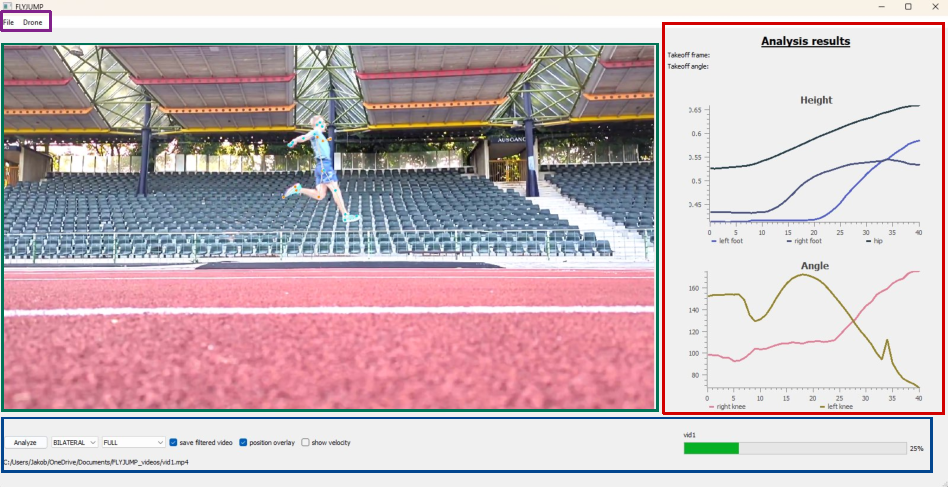
\includegraphics[scale=0.9]{GUI_running_analysis.pdf}
    \caption[Analysis \acs*{GUI}]{\acs*{GUI} shown while the video analysis
    is running.}
    \label{fig:4_gui_analysis_running}
\end{figure}
\FloatBarrier
\noindent As can be seen, the \ac{GUI} is split into three main parts.
These are marked red, green and blue respectively in above
\autoref{fig:4_gui_analysis_running}.\\
The blue area is used to let the user choose important analysis parameters and
show the analysis progress.
The parameters are the filter function to be used (see
\autoref{subsubsec:4_filter_processing}) as well as the key point detection
accuracy (see \autoref{subsec:2_mediapipe_framework}) and the output mode.
Moreover, the athlete can choose to get the velocity vector calculated and
visualized in each frame.\\\\
\noindent Above this \textit{analysis control panel}, there is the actual
video widget, which is used to display the current video according to its
current analysis progress. All analysis results, that the user chose (in the
analysis control panel) are already visualized in this stage.
Particularly, the detected position overlay (the body key points) are shown.  
Thus, a first evaluation can be performed while the analysis is still running.\\\\
\noindent On the right-hand side (red box), the actual analysis results are
visualized. In this stage, only single frame parameters are calculated and
shown. More specifically, these are knee angles, left- / right foot positions
as well as the hip height.
By updating these curves successively for each analyzed frame, an overview of 
the overall jumping progression is visualized over time.\\\\
\noindent The \ac{GUI} changes its layout slightly once the analysis is
finished to offer a more convenient way to interact with the analysis results
and their respective Parameter files (see \autoref{subsec:4_param_files}).
The \ac{GUI} layout for finished video analysis is presented in following
figure: 
\begin{figure}[h!]
    \centering
    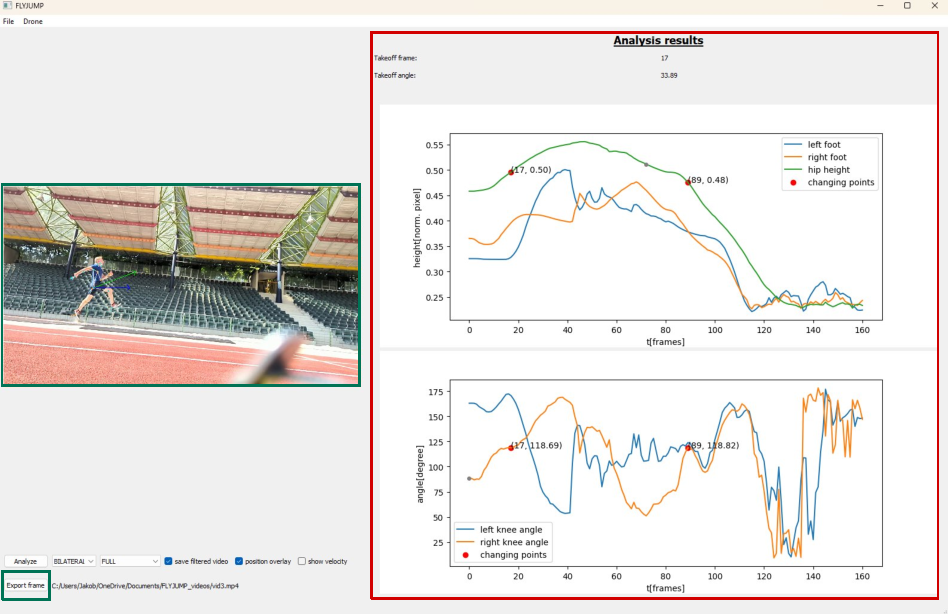
\includegraphics[scale=0.7]{GUI_finished_analysis.pdf}
    \caption[Analysis results \acs*{GUI}]{\acs*{GUI} shown once the video
    analysis is finished or a completed analysis and its corresponding
    parameter file is loaded.}
    \label{fig:4_gui_analysis_finished}
\end{figure}
\FloatBarrier
\noindent As can be seen, the analyzed video is presented in the main window (
green box in above figure).
Here, either the key points are shown as overlay over the video, or they are
shown on a black background to emphasize the posture.\\
Compared to \autoref{fig:4_gui_analysis_running} mainly the result area
changes its layout.
Especially, the full video parameters (takeoff frame- and angle) are
shown.
Moreover, the analyzed video playback starts with the automatically detected
takeoff frame on which the calculated takeoff angle (and its according
vectors) is annotated.\\
Furthermore, the analysis area now shows the complete knee angle, foot
positions and hip position plots created via the \texttt{matplotlib}
library.
Within these plots the frames corresponding to the phase transition points
(see \autoref{fig:4_long_jump_sketch}) are marked red.
Additionally, the currently visible frame is marked, too.
This ensures the user to be able to visually keep track of the jumping stage
shown in the current frame.
If hovered over plots, the full values of the plots are shown at this exact
frame number.
Once the user clicks in a plot, the video playback jumps to the selected frame
number.
This way, the athlete can jump through important parts of their total jump
according to the analyzed parameters.\\
Furthermore, the software allows exporting single video frames as images to
offer the athlete quick later access to important video frames (such as the
takeoff frame).\\\\

\noindent To allow for a convenient \ac{GUI} interaction while a video is
being analyzed or their results are presented, the video is implemented as an
own \texttt{Video} class that inherits from PyQt's \texttt{QRunnable} class.\\
Objects of this class can generally be used to either start the analysis
process or the video playback.
As the class inherits from \texttt{QRunnable}, the analysis (and the video
playback respectively) can run in a background thread which allows to keep the
\ac{GUI} responsive.
Furthermore, multiple video objects can theoretically run
concurrently\footnote{In reality, this is limited by the number of available
\ac{CPU} cores and especially by Pythons' Global Interpreter Lock (GIL)} by
using PyQt's \texttt{QThreadPool}, allowing especially to perform multiple
video analysis in parallel.
Test runs have shown that two \ac{CPU} cores per video analysis lead to the
best results when performing multiple analysis simultaneously.\\
As the video is running in a background thread, it can not directly show its'
frames in the \ac{GUI}s' main application thread.
Thus, to visualize the video frames, PyQt's signal and slot mechanisms are
used.
Whenever a video frame is ready to be visualized, the corresponding video
object emits a \texttt{visualize\_frame(Frame)} signal, where \texttt{Frame}
is a custom class that abstracts a numpy video Frame object.
The main thread has a slot to which this signal is connected.
This way, video frames are visualized by the main thread only while the
background threads are only responsible for the analysis and video loading.
The overhead introduced by using signals and slots is not considered too
large, as the \texttt{Frame} objects are passed by reference (meaning they
are not copied).\\
The interaction with the background video object is realized similarly using
signals being emitted by the main thread (e.g. abort analysis, stop playback,
jump to a specific frame,\ldots) and corresponding slots executing the actual
action in the \texttt{Video} class.


\section{Drone setup}\label{sec:4_hardware}
In order to capture high-quality video recordings that cover a complete long 
jump, from the first step all the way to the landing, a drone is used to fly
next to the athlete throughout the whole process.
Thus, a drone in form of a quadcopter is built from scratch.
Its control will be integrated seamlessly in the projects' \ac{GUI}.\\
This section introduces the hardware components that are used for building 
this drone as well as its flight control unit.\\
A short outline of the hardware is given in 
\autoref{subsec:4_hardware_selection},
while \autoref{subsec:4_hw_setup} focuses on the overall assembly of the 
selected hardware.

\subsection{Hardware selection}\label{subsec:4_hardware_selection}
Currently, commercial drone hardware on the market is mainly separable into 
the two large areas of fully remote controlled \ac{FPV} hardware and hardware 
for (autonomous) drones that can usually carry more load, e.g.~heavy cameras.
Even though the quadcopter in this project needs to be remotely 
controllable from a ground station pc, it is still more likely to be located 
in the latter one.\\
Generally the hardware was chosen based on the following criteria:
\begin{itemize}
    \item price
    \item compatibility
    \item size
\end{itemize}

\subsubsection{Flight Hardware}\label{subsec:4_filght_hardware}
The main hardware that a quadcopter needs to fly will, in the following, be
referred to as \textit{flight hardware}.
This includes frame, motors, rotors, \acp{ESC} and a \ac{PDB}.\\
The main platform on which all drone hardware is mounted, is referred to as
a quadcopter's frame.
As this project's drone does not need to carry any heavy load, such as high 
precision camera systems or other sensors, a rather compact frame would 
theoretically be sufficient.
However, compact frames tend to be less stable compared to larger frame sizes 
which could lead to a lower video recording quality and thus require more 
complex post-processing software.
Moreover, the assembly process on larger frames is more convenient and 
replacing parts is easier.
Additionally, compact frames are most commonly used in areas that demand quick
reaction times for high speed flight maneuvers, e.g.~in drone racing.
This however is not needed in this project's context.\\
Taken the mentioned considerations into account the mid-sizes \textit{Holybro 
S500 V2} frame kit is chosen.
Besides the frame, the kit also includes a landing gear and rotors.
Moreover, the main platform includes a \ac{PDB} to split the battery's power 
equally to all four motors.\\
An overview of all included parts is given in \autoref{fig:4_frame_kit}.
\begin{figure}[!h]
    \centering
    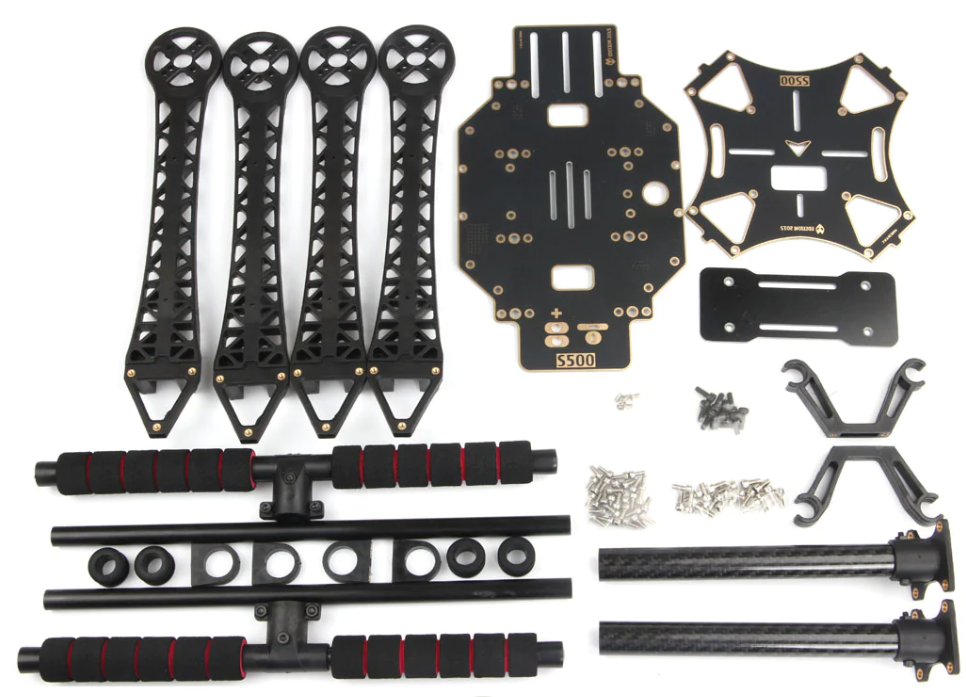
\includegraphics[scale=0.6]{frame-kit.png}
    \caption[Frame kit]{Holybro S500 V2 frame kit}
    \label{fig:4_frame_kit}
\end{figure}
\FloatBarrier
\noindent Besides the frame, motors and compatible \acp{ESC} are crucial 
flight hardware components.
Each motor requires an own \ac{ESC} that translates signals from a flight 
control unit to a voltage and thereby control the motors' rotation speed.
To guarantee compatibility, both components were chosen from Holybro as well
and can be seen in \autoref{fig:motors_and_esc}.
\begin{figure}[!h]
    \begin{subfigure}[b]{0.48\textwidth}
        \includegraphics*[scale=0.15]{motor.jpg}
        \caption{920KV Motor}
        \label{subfig:motor_picture}
    \end{subfigure}
    \hfill
    \begin{subfigure}[b]{0.5\textwidth}
        \includegraphics*[scale=0.15]{esc.jpg}
        \caption{\acl*{ESC}}
        \label{subfig:esc_picture}
    \end{subfigure}
    \caption[Motor and \acs*{ESC}]{Motor (a) and \acs*{ESC} (b)}
    \label{fig:motors_and_esc}
\end{figure}
\FloatBarrier
The drones' motors performance capabilities are defined by the number of 
\ac{RPM} they can perform per 1V input.
As can be seen in \autoref{subfig:motor_picture}, this link between 
rotation speed and input voltage is expressed in the arbitrary unit \textit{KV}.
The chosen motors are capable of rotating with a speed of 920~\ac{RPM} per 1V 
input voltage. 
Put into context, this is a common rotation speed in commercial and hobby 
drone applications.
Racing drones however, operate at motor speeds of up to 3500~KV.

\subsubsection{Control Hardware}\label{subsec:4_control_hardware}
In order to perform flight maneuvers with a quadcopter, each motor must be
controllable individually.
The calculation of the correct rotation speeds is generally performed by 
a \textit{flight control unit}.
Usually, it receives directional instructions from a remote control as input,
combines them with many parameters (e.g.~\acs{GPS} position, height over ground,
speed, etc.) and generates a (\acs{PWM}) output signal for each motor.\\
Within this project the flight controller needs to deal with two different 
inputs.
First, the ground station which can be seen as a remote control in this case.
Additionally, the drone should be able to fly autonomously next to an athlete
during their long jump training.
Here, the second input gets important.
The autonomous fly option requires the quadcopter to perform a person 
detection and therefore image processing on-board.
As the flight controller itself is not able to perform such calculations, an
additional \textit{companion computer} is required.
This companion computer will then send directional instructions just like the 
ones from the ground station to the flight controller and thereby control the 
drone.\\
The combination of flight controller and on-board companion computer will in 
the following be called \textit{control hardware}.\\
There are many types of different flight controllers available commercially.
However, most of them are not meant to be used in combination with a companion
computer.\\
Two of the most commonly used flight controllers in autonomous drone projects
are the \textit{PixHawk} and the \textit{Navio2}.
They are often chosen because they both work together seamlessly with a 
companion computer.
The former is a totally independent system which can also operate without any 
supporting computer.
The latter is implemented as \ac{HAT} specifically designed for a Raspberry 
Pi.
Thus, it does not include an own \ac{CPU} but uses the Raspberry Pis's 
resources to perform flight relevant calculations.\\
A detailed comparison between both flight controllers is given in 
\autoref{table:4_flight_cotroller_cmp}.
\begin{table}[h!]
    \centering
    \begin{tabular}[c]{|p{4cm}||p{4cm}|p{4cm}|}
    \hline
    \multicolumn{3}{|c|}{Flight Controller Comparison}\\
    \hline
    Criteria & PixHawk & Navio2\\
    \hline
    \hline
    Processor & ARM Cortex M4 with FPU / 32-bit co-processor & Depends on Raspberry
    Pi version\\
    \hline
    Sensors & ST Micro 16-bti gyroscope, ST Micro 14-bit accelerometer, MEAS
    barometer & MPU9250 9DOF IMU, LSM9DS1 9DOF IMU, MS5611 Barometer, U-blox M8N 
    Glonass/\acs{GPS}/Beidou\\
    \hline
    Interfaces & UART, Spektrum DSM, PPM / S.BUS input, I2C, SPI, CAN, USB, 3.3V 
    and 6.6V ADC input, 8 \acs{PWM} outputs, 6 Auxiliary outputs & UART, I2C, ADC, PPM / 
    S.BUS input, 14 \acs{PWM} outputs\\
    \hline
    Dimensions\newline(W x H x L) in mm & $50 \times 15.5 \times 81.5$ & $55 \times 65$\\ 
    \hline
    Other & Failsafe options (e.g. extra power supply, \acs{GPS}, etc.) & None\\
    \hline
    Price (Eur.) & TBD & TBD\\
    \hline
    \end{tabular}
    \caption[Flight controller comparison]{Comparison between PixHawk and 
    Navio2 flight controller.}
    \label{table:4_flight_cotroller_cmp}
\end{table}

\noindent As can be seen, both flight controllers offer different interfaces 
to connect additional hardware.
Moreover, both systems include sensors, mostly to gather information about 
drone's current position and inertia.
Here, the Navio2 even offers more sensors, as it already includes a \ac{GPS} 
sensor, while the PixHawk relies on an external one.\\\\
\noindent For this project, the PixHawk was chosen over the Navio2 mainly for 
three reasons.
First, it is on the market for a long time already and thus have a large 
community support.
Secondly, as it is an independent system, a failure of the companion computer 
will not lead to a crash.
Lastly, it allows for a wide range of companion computers, while the Navio2 
can only interoperate with a Raspberry Pi.\\
Furthermore, the mentioned considerations lead to easy rapid prototyping 
approaches, as the drone can be manually flown without a companion computer in
a first implementation.

\subsection{Hardware assembly}\label{subsec:4_hw_setup}
In the following, a high-level overview of the quadcopters' hardware setup is 
given.
The general wiring is shown and explained before a short introduction of some 
important communication protocols is given.

\subsubsection{General wiring}
In the following \autoref{fig:4_general_wiring} the general wiring layout is 
shown.
The whole system is powered from one power source only.
\begin{figure}[!h]
    \centering
    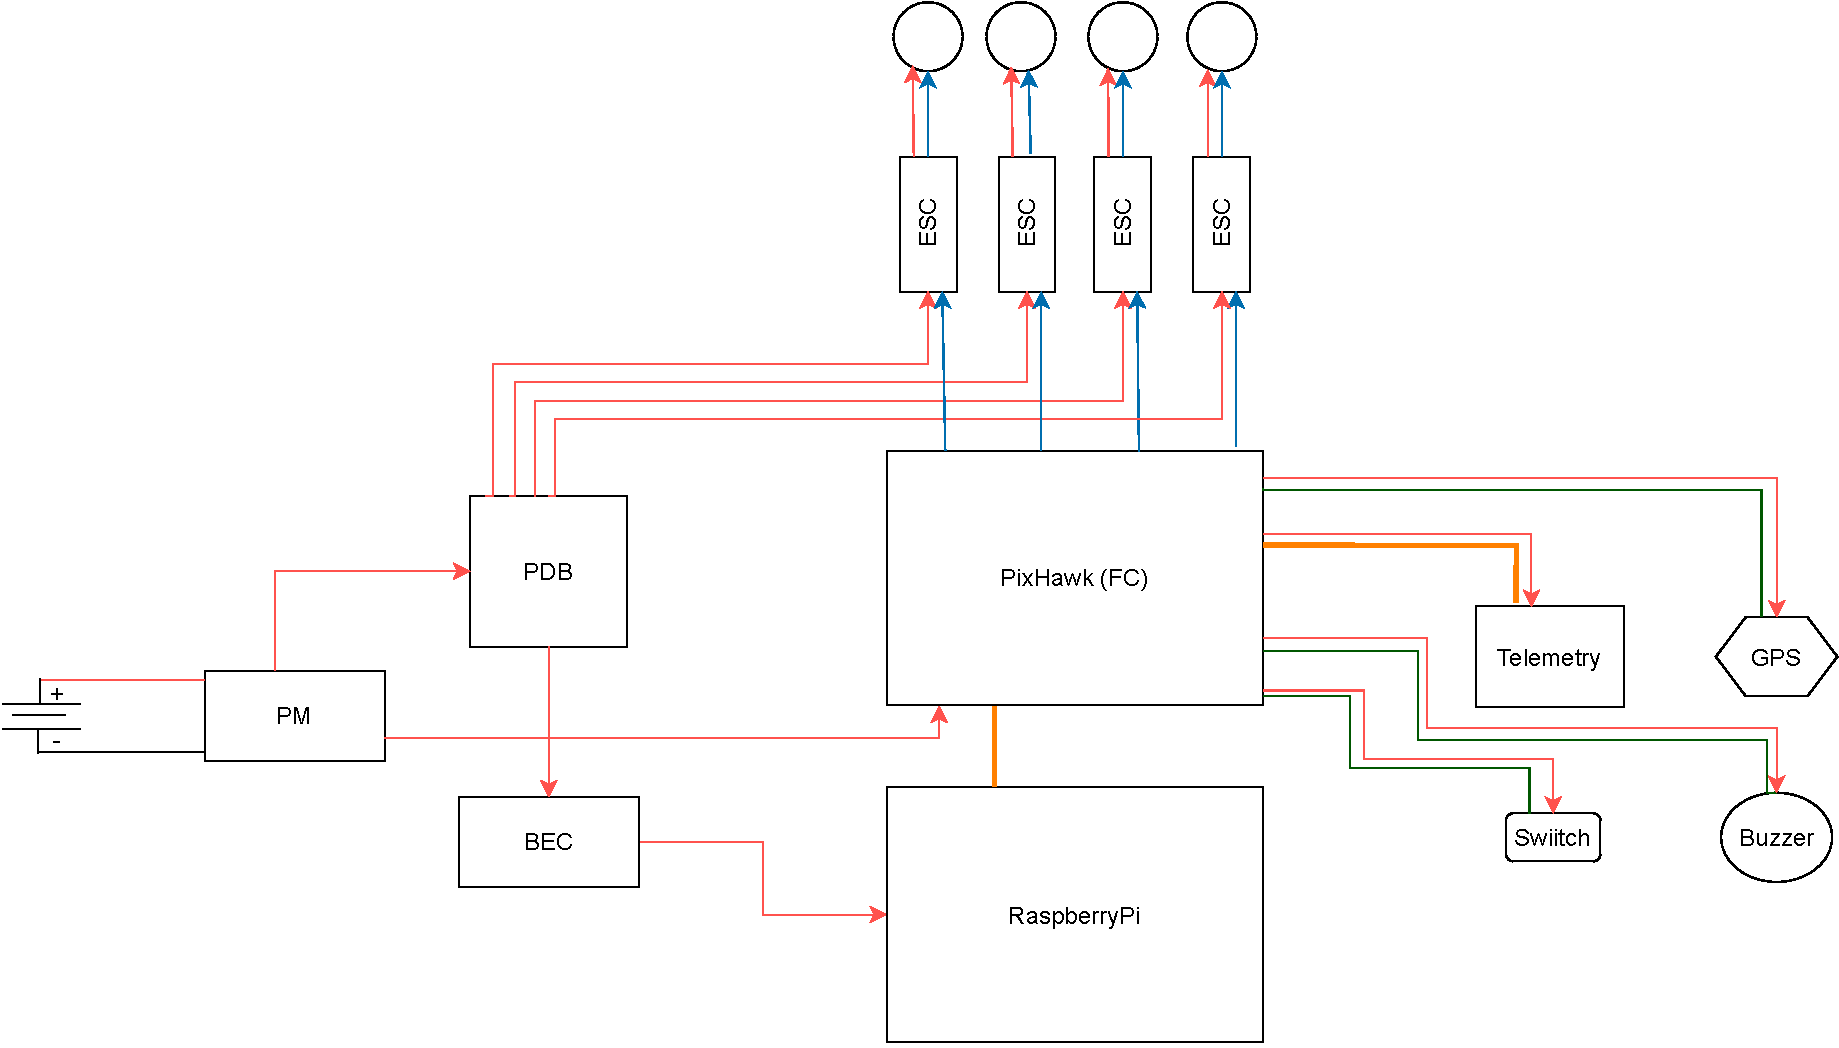
\includegraphics[scale=0.5]{general_wiring.pdf}
    \caption[General Wiring]{General wiring of the hardware setup.\\
    Power connections are labeled red, 
    Blue connections are used for \ac{PWM} signals, 
    Green connections are serial connections, 
    orange connections are more specifically serial UART connections.}
    \label{fig:4_general_wiring}
\end{figure}
\FloatBarrier
\noindent This results in some challenges in providing the correct voltage for
each connected device.
In the current setup this task is taken over by three devices.
The \ac{PM} is directly connected to the battery.
It transfers the battery's voltage to the \ac{PDB} and a lower 5V voltage to
the PixHawk flight controller.
The \ac{PDB} itself is a parallel circuit, thus providing the same voltage
(battery voltage) to each output.
The third device is a \ac{BEC} which is directly connected
to the \ac{PDB} and delivers a constant 5V output.
This can be used to power a companion computer such as a RaspberryPi.\\
All other required peripherals are powered by the PixHawk flight controller
itself.
The main peripherals used in this project are a telemetry module which is used
for communication with a ground station and a \ac{GPS} module used for
improving the drones capabilities to follow a defined trajectory, which is
specifically useful for auto-return~and landing features.
Two more peripherals, a buzzer to output audio warning signals and a manual
kill switch which can immediately stop all four motors, are installed mainly
for safety reasons.\\
The hardware components that actually control the motor rotation speeds,
the \acp{ESC}, are connected to the \ac{PDB} for power supply as well as to
the flight controller that calculates the correct rotation speeds based on the
wanted flight maneuvers and outputs a \ac{PWM} signal for each motor.\\
The presented overall wiring is rather complex but allows relying on one power
source only instead of using multiple power sources for flight hardware and
control hardware including peripherals respectively.

\subsubsection{Communication between components}\label{subsec:4_comm}
The drone setup needs hardware components to communicate with each other in 
order to transfer control signals from either the companion computer or from
the ground station to the flight controller.
Even if both options origin from different sources, they use the same
device-to-device communication protocol.
The protocol used for this purpose is the \textit{UART} protocol, which is
acronym for universal asynchronous receiver / transmitter protocol.
It is based on a serial, full duplex connection using six connections.
The connection layout is shown in \autoref{fig:4_uart_wiring},
\begin{figure}[!h]
    \centering
    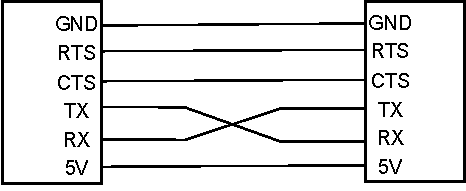
\includegraphics[scale=0.8]{uart_wiring.pdf}
    \caption[UART wiring]{UART wiring}
    \label{fig:4_uart_wiring}
\end{figure}
\FloatBarrier
\noindent where RTS / CTS denote Ready to send and Clear to send.
RX / TX represent the actual data receiving and sending connections
respectively.\\

\noindent UART transfers data using data frames with minimal overhead.
A typical UART frame consists of just a start bit, data bits, a parity bit and
a stop bit.
\autoref{fig:4_uart_frame} visualizes such a data frame. 
\begin{figure}[!h]
    \centering
    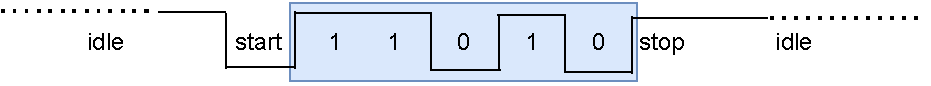
\includegraphics[scale=0.8]{uart_frame.pdf}
    \caption[UART data frame]{Exmple of an UART data frame. The blue marked
    area is the actual data part that is transmitted.}
    \label{fig:4_uart_frame}
\end{figure}
\FloatBarrier
\noindent The shown UART data frame includes 5 data bits, however, the amount
can vary between 5 and 9.
Moreover, the included even parity bit is optional.
The idle state is set to a voltage that represents HIGH level on purpose, so
that any connection failure is easily detectable.
UART can work with any voltages to denote HIGH and LOW levels.
In the quadcopter setup HIGH is represented by 5V and LOW by GND.

\section{Controlling the drone}\label{sec:4_drone_ctrl}
Besides starting the measurement recordings and analyzing the recorded jumps,
the ground station is also used to align the drone next to the athlete.
Hence, a basic drone control is implemented supporting fundamental movements
including forward, backward, left, right, ascending, descending, and rotation
(around the drone's vertical axis).\\
The control in this work is based on the MAVLink
protocol~\cite{koubaaMicroAirVehicle2019} and the
corresponding python library \texttt{pymavlink} which is able to send and
receive MAVLink messages (e.g. via a serial interface).\\
All MAVLink packets follow the same structure\footnote{This work uses MAVLink
v2. Thus, only this version's packet structure is shown.}:
\begin{figure}[!h]
    \centering
    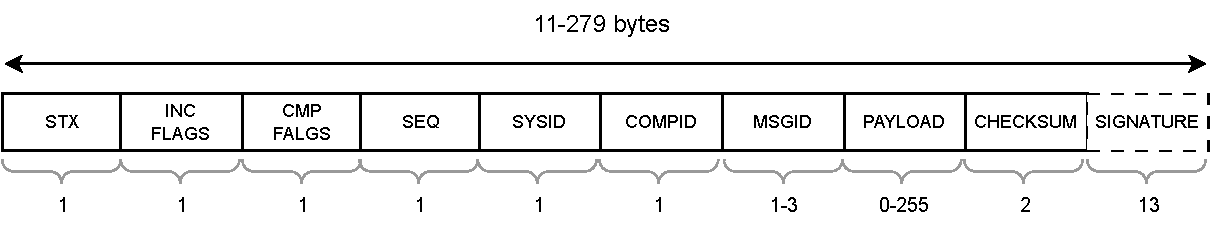
\includegraphics[scale=0.7]{mavlink_v2.pdf}
    \caption[Structure of a MAVLink message]{Structure of a MAVLink message.\\
    Below each component, their respective size in bytes is shown.\\
    The signature is optional.\\
    The visualization is based on the MAVLink 2.0 header shown
    in~\cite{koubaaMicroAirVehicle2019}}
    \label{fig:4_mavlink_message}
\end{figure}
\FloatBarrier
\noindent As this work does not use message signatures, the shown packet
structure leads to a (maximal) message size of 266 bytes\footnote{11 bytes
overhead + 255 bytes payload}.
Due to its low overhead (11 bytes), the protocol is considered lightweight and
is therefore used in many applications where low latencies are important.
However, the protocol therefore does not include any security measures (apart
from the message signature) like encryption.\\
In the following, each part belonging to the drone control process, namely
the connection and the movement control is explained based on the above shown
MAVLink message structure.

\subsection{Connection}\label{subsec:4_drone_conn}
The control-connection between the drone and the ground station is established
using two SiK telemetry radios operating at a frequency of 433~MHz with a
transmission power of 100~mW.
One is mounted on the drone and is directly connected to the PixHawk flight
controller (see \autoref{fig:4_general_wiring}), the other one is connected
to the ground station using a serial connection (USB), respectively.\\
As MAVLink is a connectionless protocol~\cite{atoevDataAnalysisMAVLink2017},
no permanent connection is established.
However, as it is important to know whether the drone is still reachable by
the ground station, a heartbeat signal is used to ensure a connection.
Thus, the terminus \textit{connected} will in the following be used, if a
heartbeat is received from the drone.
Otherwise, the drone is considered \textit{disconnected}.\\
Besides receiving a heartbeat signal from the drone, the ground station emits
one itself, too.
By this combination of exchanging heartbeats between the two systems, a correct
connection is ensured.\\
The camera and thus, video recording control is discussed separately in
\autoref{subsubsec:4_pi_wifi} (and following).\\\\
\noindent Implementation wise, the heartbeat connection is handled in an own
thread.
Thus, the connection is kept alive in background while the \ac{GUI} stays
responsive to handle user interaction.
The heartbeat is sent at a frequency of 1~Hz by the ground station and the
flight controller respectively.
Hence, the worst case time for detecting a connection loss lies at 1~sec.
Once the heartbeat thread is started, heartbeats are sent until either the
thread gets interrupted or a connection timeuout occured:

\begin{pythoncode}[caption=Sending mavlink heartbeats,label=alg:heartbeat_mav_send]
    def emit_heartbeat():
        system_type = mavutil.mavlink.MAV_TYPE_GCS
        autopilot_type = mavutil.mavlink.MAV_AUTOPILOT_INVALID
        while True:
            self.connection.mav.heartbeat_send(
                system_type,
                autopilot_type,
                0,  # MAV_MODE_FLAG
                0,  # Custom mode, not used for FLYJUMP
                0,  # System status, not used for for FLYJUMP
                0,  # MAVLink version, 0: default(2.0)
            )
            time.sleep(1)
\end{pythoncode}
The provided code example uses \texttt{time.sleep(1)}.
Thus, the background thread executing this function is scheduled as few as
possible, ensuring that it consumes as little \ac{CPU} time as possible.
Moreover, the communication channel does not get overloaded.
The used \texttt{heartbeat\_send} function is provided by the
\texttt{pymavlink} library.
The system type is set to indicate the heartbeat's origin, which is the ground
station in this case.
The parameter \texttt{MAV\_AUTOPILOT\_INVALID} indicates that the heartbeat is
sent by a system without any autopilot software installed.\\\\
\noindent The heartbeat receiving part is implemented using \texttt{pymavlink}
, too.
It is handled within the same thread as the heartbeat emitting.
Hence, both functionalities are abstracted in a \texttt{DroneConnection} class
which inherits from \texttt{Qhread} to make it executable in a background
thread.\\
To receive heartbeats from the drone, the \texttt{recv\_match()} function is
used.
This function can generally receive (wait for) every MAVLink message
available.
Furthermore, it can either be executed synchronously or asynchronously.
The heartbeat receiving relies on the asynchronous version.
If the time between two consecutive heartbeat signals exceeds two seconds, the
connection is considered to be lost.
The usage of asynchronous receiving ensures, that heartbeats get emitted in
regular intervals and are not blocked by the receiving function.

\subsection{Movement}\label{subsec:4_drone_mvmnt}
Once a conrol-connection is established (see above
\autoref{subsec:4_drone_conn}), the drone software supports basic movements to
control the drone.
All supported movement instructions are sent via the MAVLink protocol using
the \texttt{pymavlink} module.
Moreover, all messages are sent from a background thread.
The corresponding thread is generally setup similarly to the aforementioned
drone connection thread, now however, the supported movements are
abstracted in one \texttt{DroneControl} class, which inherits from
\texttt{QThread}.
Furthermore, it needs a valid\footnote{Drone connection objects become
invalid whenever the connection to the drone gets interrupted.} 
\texttt{DroneConnection} object to work.\\\\
\noindent In the following the drone control is explained using multiple
coordinate systems, also referred to as coordinate frames.
The axis are therefore denoted as following: the y-axis represents the
horizontal axis, the z-axis denotes the vertical axis and the
x-axis denotes the axis orthogonal to both of them.\\
All movements are implemented using MAVLink's
\texttt{SET\_POSITION\_TARGET\_LOCAL\_NED} message, which allows to control
the drone relative to either its' takeoff location or its current position.
The term NED indidcates the previously defined \textbf{N}orth (X-axis),
\textbf{E}ast (Y-axis), \textbf{D}own (Z-axis) coordinate frame.\\
However, this coordinate frame only defines the movement directions (e.g. 2~m
in positive Z-direction means descending by 2~m), it does not define the it's
origin.
Furthermore, it does not define if the axis directions stay fixed (e.g. the
X-axis always points to the north) or if they are relative to the drone (e.g.
the X-axis points to the drone's front).
Each of the aforementioned coordinate frame options are supported by Ardupilot. %TODO: mention Ardupilot before
Thus, in order to achieve the desired movement, the according coordinate
frame needs to be provided\footnote{In reality, the coordinate frames are
stored on the flight controller.
Each one has a unique ID which can then be referred to.} each time a movement
command is sent.
All three aforementioned coordinate frames are shown in following
\autoref{fig:4_control_coord_frames}:
\begin{figure}[htbp]
    \centering
    \begin{subfigure}{0.45\textwidth}
        \centering
        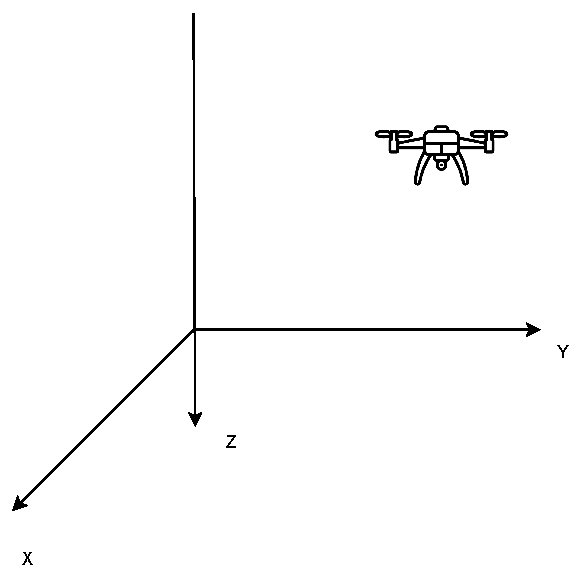
\includegraphics[width=\linewidth]{coordinate_frame_global.pdf}
        \caption{Global coordinate frame with the origin fixed to the drone's
        takeoff location.}
    \end{subfigure}\hfill
    \begin{subfigure}{0.45\textwidth}
        \centering
        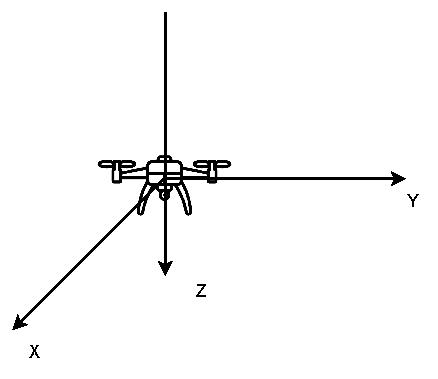
\includegraphics[width=\linewidth]{coordinate_frames_local.pdf}
        \caption{Local coordinate frame with the origin moving with the
        drone's current position.}
    \end{subfigure}
    \caption[Drone movement coordinate systems]{Coordinate frames used for
    movement commands.}
    \label{fig:4_control_coord_frames}
\end{figure}

\begin{figure}[htbp]
    \ContinuedFloat
    \centering
    \begin{subfigure}{1.0\textwidth}
        \centering
        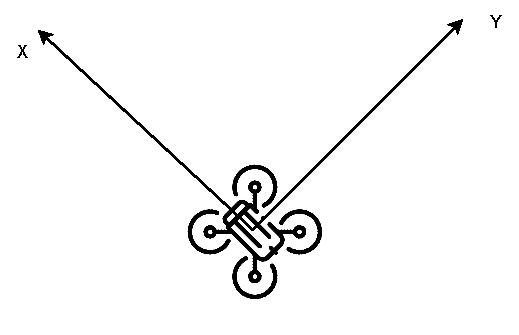
\includegraphics[scale=0.8]{coordinate_frames_local_heading.pdf}
        \caption{Local coordinate frame with the origin moving with the
        drone's current position and the axis orientation rotating according
        to the drone's heading. Z-Axis pointing downwards.}
    \end{subfigure}
    \caption*{Coordinate frames used for movement commands (continued).}
\end{figure}
\FloatBarrier
\noindent As the drone flies alongside the athlete with an arbitrary approach
length, the absolute coordinate offset between the drone's takeoff point
and the point where the jump is complete is unknown.
Thus, the global coordinate frame (a) is not suitable for this work.
The local coordinate systems (b) and (c) however, can both be used to align
the drone alongside the athlete during the jump.
They only differ in the way the movements are executed.
When using coordinate frame (b), the drone always turns into the direction it
is flying (e.g. flying 1~m north leads to turning the drone's front north and
then flying 2~m along the noth axis).
As coordinate frame (c) consinders the drone's current heading the same
command here leads to flying 2~m forward (to the drone's north).\\\\
Following code is used to control the drone according to coordinate frame (b):

\begin{pythoncode}[caption=Movement commands using local\_ned,label=alg:send_ned_command]
    def ned_command(self, x, dx, d2x):
        self.connecion.send(
            mavutil.mavlink.MAVLink_set_position_target_local_ned_message(
                0, target_system, target_component,
                9, # frame id
                int(0b110111000111), #bitmask
                *x, #(x, y, z) in m
                *dx, #(x, y, z) velocity in m/s
                *d2x, #(x, y, z) velocity in m/s^2
                0, 0 #yaw (rad), yaw rate (rad/s)
            )
        )
\end{pythoncode}
As can be seen in above code example, the drone can be controlled according to
either a position offset, a velocity or an acceleration.
In this work, especially the velocity option is important.
Hence, the drone can fly next to an athlete matching their run-up speed.
The above shown example is set-up as an example for velocity control.
However, the control based on other parameters is similar.\\
In above example, the bitmask \texttt{0b110111000111} is used to enable (or
disable) the provided paramters (in this exact order: position, speed,
acceleration, yaw angle and yaw rate).
The bitmask is setup from right to left, meaning the rightmost bit enables/
disables the provided x position offset.
Furthermore, the bitmask is inverted.
Thus, a 1 disables the parameter (according to its position) and a 0 enables
it respectively\footnote{Bit 10 (from the right) is unused by the system.}.
The shown \texttt{self.connection} is an instance of the
\texttt{DroneConnection} class, allowing the commands to be sent in background
thread.\\\\
\noindent All message parameters shown are embeddded in the MAVLink message
protocol (see \autoref{fig:4_mavlink_message}).
As response to the sent movement commands, the drone replies with an
acknowledge message including the original movement command.
Hence, the acknowledgement is received asynchronously by the ground station.\\\\
\noindent The supported movements (forward, backward, left, right, ascending,
descending and rotation around the z-axis) are triggered by either the
\ac{GUI} (see \autoref{subsec:4_drone_ctrl_panel_gui}) or the keyboard.
Here, \textit{WASD} is used for North (X), East (Y) movements and
\textit{IJKL} is used for Down (Z) and yaw movements.
The keyboard interection is therefore captured by the software's main thread.
Then, signals are sent to the background thread's slots to trigger the command
sending shown above.
If the user holds one of the keys, the according movement control message is
sent at a frequency of 1~Hz, allowing for a smmooth flight path\footnote{If
the drone does not receive a control message for two seconds, it automatically
stops and loiters at it's current position.}. 

\subsection{GUI control panel}\label{subsec:4_drone_ctrl_panel_gui}
As aforementioned, the drone control as well as drone status messages (e.g.
GPS satelite count, errors) and the camera live-stream (
\autoref{subsec:4_rec_stream_video}) are combined into one \ac{GUI} control
panel, allowing for a convenient drone - ground station interaction.
Thus, as long as the control panel is openend, the \ac{TCP} connection (used
for camera control) and the control connection (via MAVLink) is kept alive.\\
The control panel is shown in \autoref{fig:4_drone_ctrl_panel}:
\begin{figure}[!h]
    \centering
    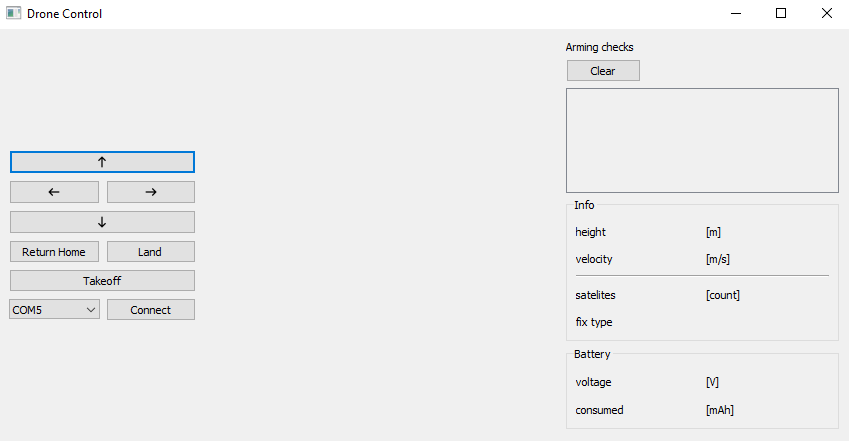
\includegraphics[scale=0.6]{drone_control_panel.png}
    \caption[Drone control panel]{Drone control panel}
    \label{fig:4_drone_ctrl_panel}
\end{figure}

\noindent The shown control panel is divided into three main areas, namely a
connection control area, a video control area and a drone status area (from
left to right).
The serial port to which the telemetry radio is connected, is automatically
detected.
To allow for a quick takeoff- and landing process, according quick-action
buttons are implemented.
Especially the \textit{return to home} function is helpful as no manual user
interaction is required to land the drone at the exact takeoff location.
The automatically detected telemetry port is then used to establish the
control connection to the drone once the \textit{connect} button is clicked.
The connect button triggers the \ac{TCP} streaming connection, too.
The received camera live-stream is then shown in the middlle section of the
control panel.\\
On the panel's right side, the drone's current status is shown.
This includes the \ac{GPS} condition as well as the most important filght
parameters (height over ground and velocity over ground).
Furthermore, the battery status is shown for safety reasons.\\
The upper part in the status area is reserved for important messages from the
drone (e.g. when some commands are rejected or some internal failure occurs).
The status message report needs to be requested explicitly, which is done in
combination with receiving the drone's heartbeat (see
\autoref{subsec:4_drone_conn}) at a frequency of 1~Hz.

\section{Drone camera control}\label{subsec:4_live_stream}
As the drone is meant to be used to support the long jump analysis process by
recording the jump and sending the captured video to a ground station, a
complete video recording process is developed and implemented.\\
This includes the hardware camera setup on the drone, as well as the
communication between the ground station which initializes the video
recording and the drone capturing the actual video.\\
Generally, the on-board RaspberryPi takes care of capturing the video
recordings.
It starts the video recording when it is triggered via the ground station and
sends the recorded video file back to the ground station after the recording
has ended.
The video is then analyzed on the ground station.
Moreover, the RaspberryPi offers a live stream of the current camera image to
allow for aligning the drone correctly relative to the athlete.\\
In the following, the implementations of the aforementioned features are shown
in detail.

\subsection{Connection between the ground station and the on-board computer}\label{subsec:4_pi_wifi}
In order to start or stop video recordings or capture images as well as to
send video recordings back to the ground station, the on-board mounted
RaspberryPi needs to communicate with the ground station.
Furthermore, this connection is used to stream live images from the drone to
the ground station, too.\\
There are many implementations that use
analog~\cite{tecpoyotl-torresRealtimeVideoTransmission2021} video transmission
for live-streaming videos from \ac{FPV} drones.
More recently, digital alternatives~\cite{silicQoEAssessmentFPV2021} with
comparable latencies were developed.
However, the live stream in this work is meant to be used for aligning the
drone only, not for controlling it.
Thus, the real-time requirements are less important.
Furthermore, the connection is not only used to live-stream videos, but also
to send commands (e.g. start video recording) and video files.
Hence, the connection to the on-board computer is realized using a Wifi
network.
This is achieved by setting up the RaspberryPi as access point to which the
ground station can then connect directly.\\
This creates an arbitrarily useable connection which allows for quick
transmission speeds.
As the ground station and the drone are always used together on-field (which
guarantees physical proximity), the limited Wifi transmission range is not
considered as problematic for the following Implementations.

\subsubsection{TCP sockets for communication}\label{subsubsec:4_tcp_sockets}
Even though the video recording is performed by the on-board RaspberryPi, the
recording must be initializable by the user via the ground station.
Therefore, the communication between these two computers is established using
a \ac{TCP}~\cite{cerfProtocolPacketNetwork1974} connection.
As potentially large video files are transferred wirelessly from the
RaspberryPi to the ground station, a connection-orientated and confirmed
\ac{TCP} connection protocol is chosen over a connectionless
\ac{UDP}~\cite{SpecificationInternetTransmission1974} to avoid data loss.\\\\

\noindent When the ground station connects to the drone, a \ac{TCP} socket is
opened in a background thread.
The corresponding \ac{TCP} connection is initialized by the
ground station using a three-way handshake\footnote{The request is sent by the
ground station, the drone acknowledges, and the ground station acknowledges
the drone's response}.
To create the socket, Python's \texttt{socket} module is used to access the
BSD socket interface.
Generally, a \ac{TCP} socket is uniquely defined by an IP-Address and the
corresponding port number.
As the ground station is directly connected to the RaspberryPi's own WLAN, the
socket's IP address is equivalent to the ground station's standard gateway.
The port is set arbitrarily.\\
To start / end video recordings, pre-defined messages are sent via the created
\ac{TCP} socket.
The messages are utf-8 encoded and sent using Python's
\texttt{socket.sendAll(message)} function.
The drone on the other connection end uses \texttt{socket.recv()} to listen to
any messages sent via the \ac{TCP} connection.
If a message contains one of the pre-defined keywords (e.g.
\textit{start\_recording}, \textit{end\_recording}), the corresponding action
is executed.
The \ac{TCP} socket on the RaspberryPi for receiving control messages is set
up as shown in following Listing:
\begin{pythoncode}[caption=create TCP socket, label=alg:create_tcp_port]
    def create_socket(port: int):
        with socket.socket(socket.AF_INET, socket.SOCK_STREAM) as sock:
            sock.bind(('0.0.0.0', port))
            sock.listen()
            conn, addr = sock.accept()
\end{pythoncode}
In the above listing, the option \texttt{SOCK\_STREAM} defines a \ac{TCP}
connection.
Furthermore, the option \texttt{'0.0.0.0'} is set as IP address, instructing
the RaspberryPi  to listen for connections on all available network interfaces
(on the given port in the provided example).
Hence, any ground station can simply connect to this port to send
control instructions.\\
Some more options which are not explicitly shown are set to avoid multiple
connections being established on the same port on the one hand but allow a
connection to be re-established when it gets disconnected unexpectedly on the
other hand.\\\\
\noindent Once a video recording has ended (either because the user manually
ended the recording, or because a timeout / error occurred on the
RaspberryPi's side), the temporarily saved video is transferred to the ground
station.
This process is implemented using \ac{TCP} sockets, too.
The transmission is initiated by the on-board RaspberryPi.
The overall process is similar to the message sending part previously
explained.
Now however, the drone uses \texttt{socket.sendAll()} iteratively to send the
video divided into several chunks of 1024 byte size.
The ground station on the other hand uses \texttt{socket.recv(1024)} to
receive the video data chunks.
Once the video is completely transferred, the according file is deleted from
the on-board computer and the drone is able to record a new video again.\\
An overview of the control flow which is used to start a measurement recording
is presented in following \autoref{fig:4_measurement_ctrl_flow}.\\
\begin{figure}[h!]
    \centering
    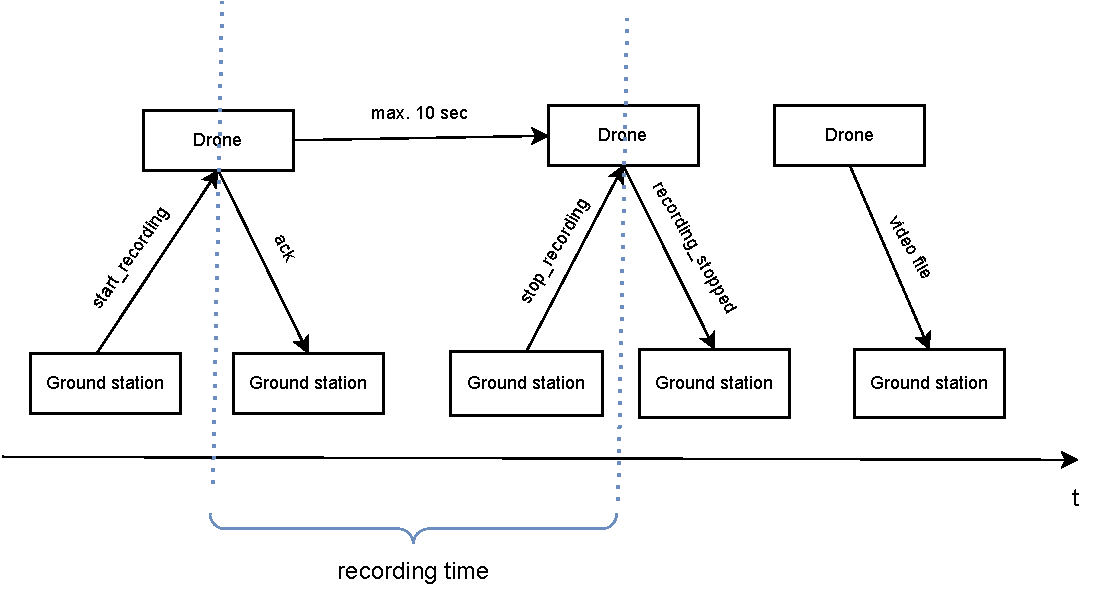
\includegraphics[scale=0.7]{request_flow.pdf}
    \caption[Measurement control flow between ground station and drone]{
        Measurement control flow between the ground station and the drone}
    \label{fig:4_measurement_ctrl_flow}
\end{figure}
\noindent It can be noted that the maximal recording time is limited to 10
seconds.
This ensures quick transfer times when the video is being sent to the ground
station.
Moreover, the implemented takeoff detection performs best on short video
sequences (see \autoref{subsec:4_runtime_performance}).\\
The timeout is set to 10 seconds, as a normal long jump usually does not take
longer than around seven\footnote{Approach length: 40 m, average run up speed:
$6.5\frac{m}{s}$, flight time: $1\sec$ leads to about $7\sec$ total jumping
time} seconds.

\subsubsection{Camera setup and video recording}\label{subsubsec:4_cam_setup_recording}
Once the RaspberryPi receives the control message to start the video
recording, the live-stream (see below \autoref{subsubsec:4_live_stream}) is
interrupted. 
Afterwards, the video recording is started.
The captured video frames are saved to a temporary .mp4 file located on the
on-borad RaspberryPi itself.
Thus, the full available frame rate and resolution can be used to record the
long jump.\\
A frame rate of 60~\ac{FPS} or higher ensures that every phase of the
jump, in particular the takeoff phase, is well resolved in the time domain.
The video is recorded at a resolution of $1920 \times 1080$ pixels.
This resolution is sufficient for the mediapipe framework to fully recognize
the athlete's posture and joints.\\\\
\noindent The camera used in this work to record long jumps is the RaspberryPi
HQ camera in combination with a 16 mm C-Mount tele lens.
The tele lens allows the drone to keep a safety distance to the athlete
during the run-up while still keeping the athlete in focus. 
To manage the video recording parameters and directly interact with the
camera, the Linux library \texttt{libcamera} is utilized, while the
\texttt{Picamera2} Python library, built upon \texttt{libcamera}, offers a
more accessible interface for this purpose.\\
Picamera2 especially offers the \texttt{create\_video\_configuration} function
to conveniently set video recording parameters such as frame rate, resolution,
or the option to rotate the captured frame in-place. 
Latter one is especially useful in this work, as the camera can thereby be
mounted to the drone in any orientation while the recorded video is still
orientated correctly.
The video frames in this work only need to be rotated by a (multiple of)
$90^{\circ}$, as the camera is not mounted at some arbitrary diagonal angle. 
Thus, the required computations can be represented by simply moving each
video frame's matrix elements to a pre-defined index.
A $90^{\circ}$ rotation e.g. is performed by simply transposing the matrix
(in-place) and reversing each row afterwards (applied to each RGB input channel
respectively)~\cite{godardEfficientOutofCoreOutofPlace2021}.\\
These transformations are performed before the video frame is written to
the actual video file.
Hence, the post-processing overhead is significantly reduced.

\subsection{Handling the incoming video live-stream}\label{subsubsec:4_live_stream}
In addition to the video recording, a live-streaming video option is
implemented to allow for aligning the drone alongside the athlete with the
athlete being centered in the camera image.\\
The live-stream is implemented similar to the implemented communication
control flow described earlier (\autoref{subsubsec:4_tcp_sockets}).
However, package loss in this case is not as relevant as it is in the
communication protocol.
Hence, the live-stream is based on \ac{UDP} sockets instead of \ac{TCP}
sockets.\\
As \ac{UDP} is connectionless, no overhead is introduced by connection
establishment or re-transmitting lost packages.
This however leads to some video frames getting (potentially) lost, which is
acceptable in this case, as the video stream is not meant to be used to
control the drone in real time.\\
To reduce the used transmission bandwidth further, the live-stream resolution
is additionally limited to $640 \times 480$ pixels.
The specific streaming parameters are again set using \texttt{Picamera2}'s
\texttt{create\_video\_configuration} function as explained in the
\hyperref[subsubsec:4_cam_setup_recording]{video recording paragraph}.
To allow for higher resolution video recording, the live-stream is not
available while a video recording is active.\\\\
\noindent On the ground station's side, the receiving is implemented using
openCV's \texttt{VideoCapture} function which can be called with the
RaspberryPi's IP address and the corresponding port number as arguments.
The received video frames are wrapped in the custom \texttt{Frame} class which
is already used in the video analysis process.
Thus, the incoming video frames could be directly analyzed.
The received video frames are then visualized using the same signal and slot
mechanisms as explained in \autoref{subsec:4_lj_software_gui}.
In order to allow for aligning the drone next to the athlete, the video stream
is shown in the \hyperref[sec:appendix_livestream]{control panel}.